\chapter{Mechanics}

\section{Overview}

\paragraph{} OpenCombat is a free and open-source 2D platform fighting game where players punch, kick, grab, block, dodge and use their super powers to knock out all their opponents in intense and fast-paced battles across diverse arenas. Players can embrace the chaos by fighting 4v4 free-for-alls with items \textit{(generously provided by the audience)} or show off their skills in competitive 1v1 matches; the rules are completely customizable in both offline and online play. Players can also create their own combatants and choose from 1 of 4 different classes each with their own unique set of moves. By completing objectives and playing matches, players will earn badges that they can proudly display on their profile.

\paragraph{} At the core of OpenCombat is the players and their experiences inside and outside the game. OpenCombat is free and all subsequent updates will also be free requiring no monthly subscriptions or purchases to acquire new content. Since the game is open source, players can create plugins or take part in helping to add new features, fix bugs or balance gameplay. One of the essential experiences of fighting games is coming together with others and playing multiplayer locally; players can use the in-game community organizing tool to host or attend events in their area.

\begin{figure}[h!]
    \centering
    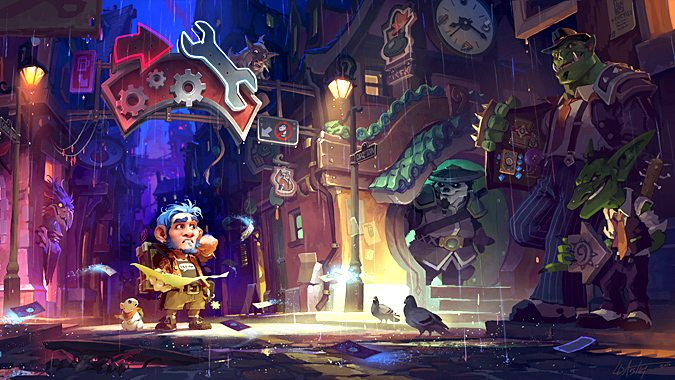
\includegraphics[width=1\linewidth]{images/setting-populated.jpg}
    \caption{Mean Streets Key Art by Blizzard Entertainment, Inc.\nocite{blizzard_entertainment_inc_mean_2016}}
\end{figure}

\begin{figure}[h!]
    \centering
    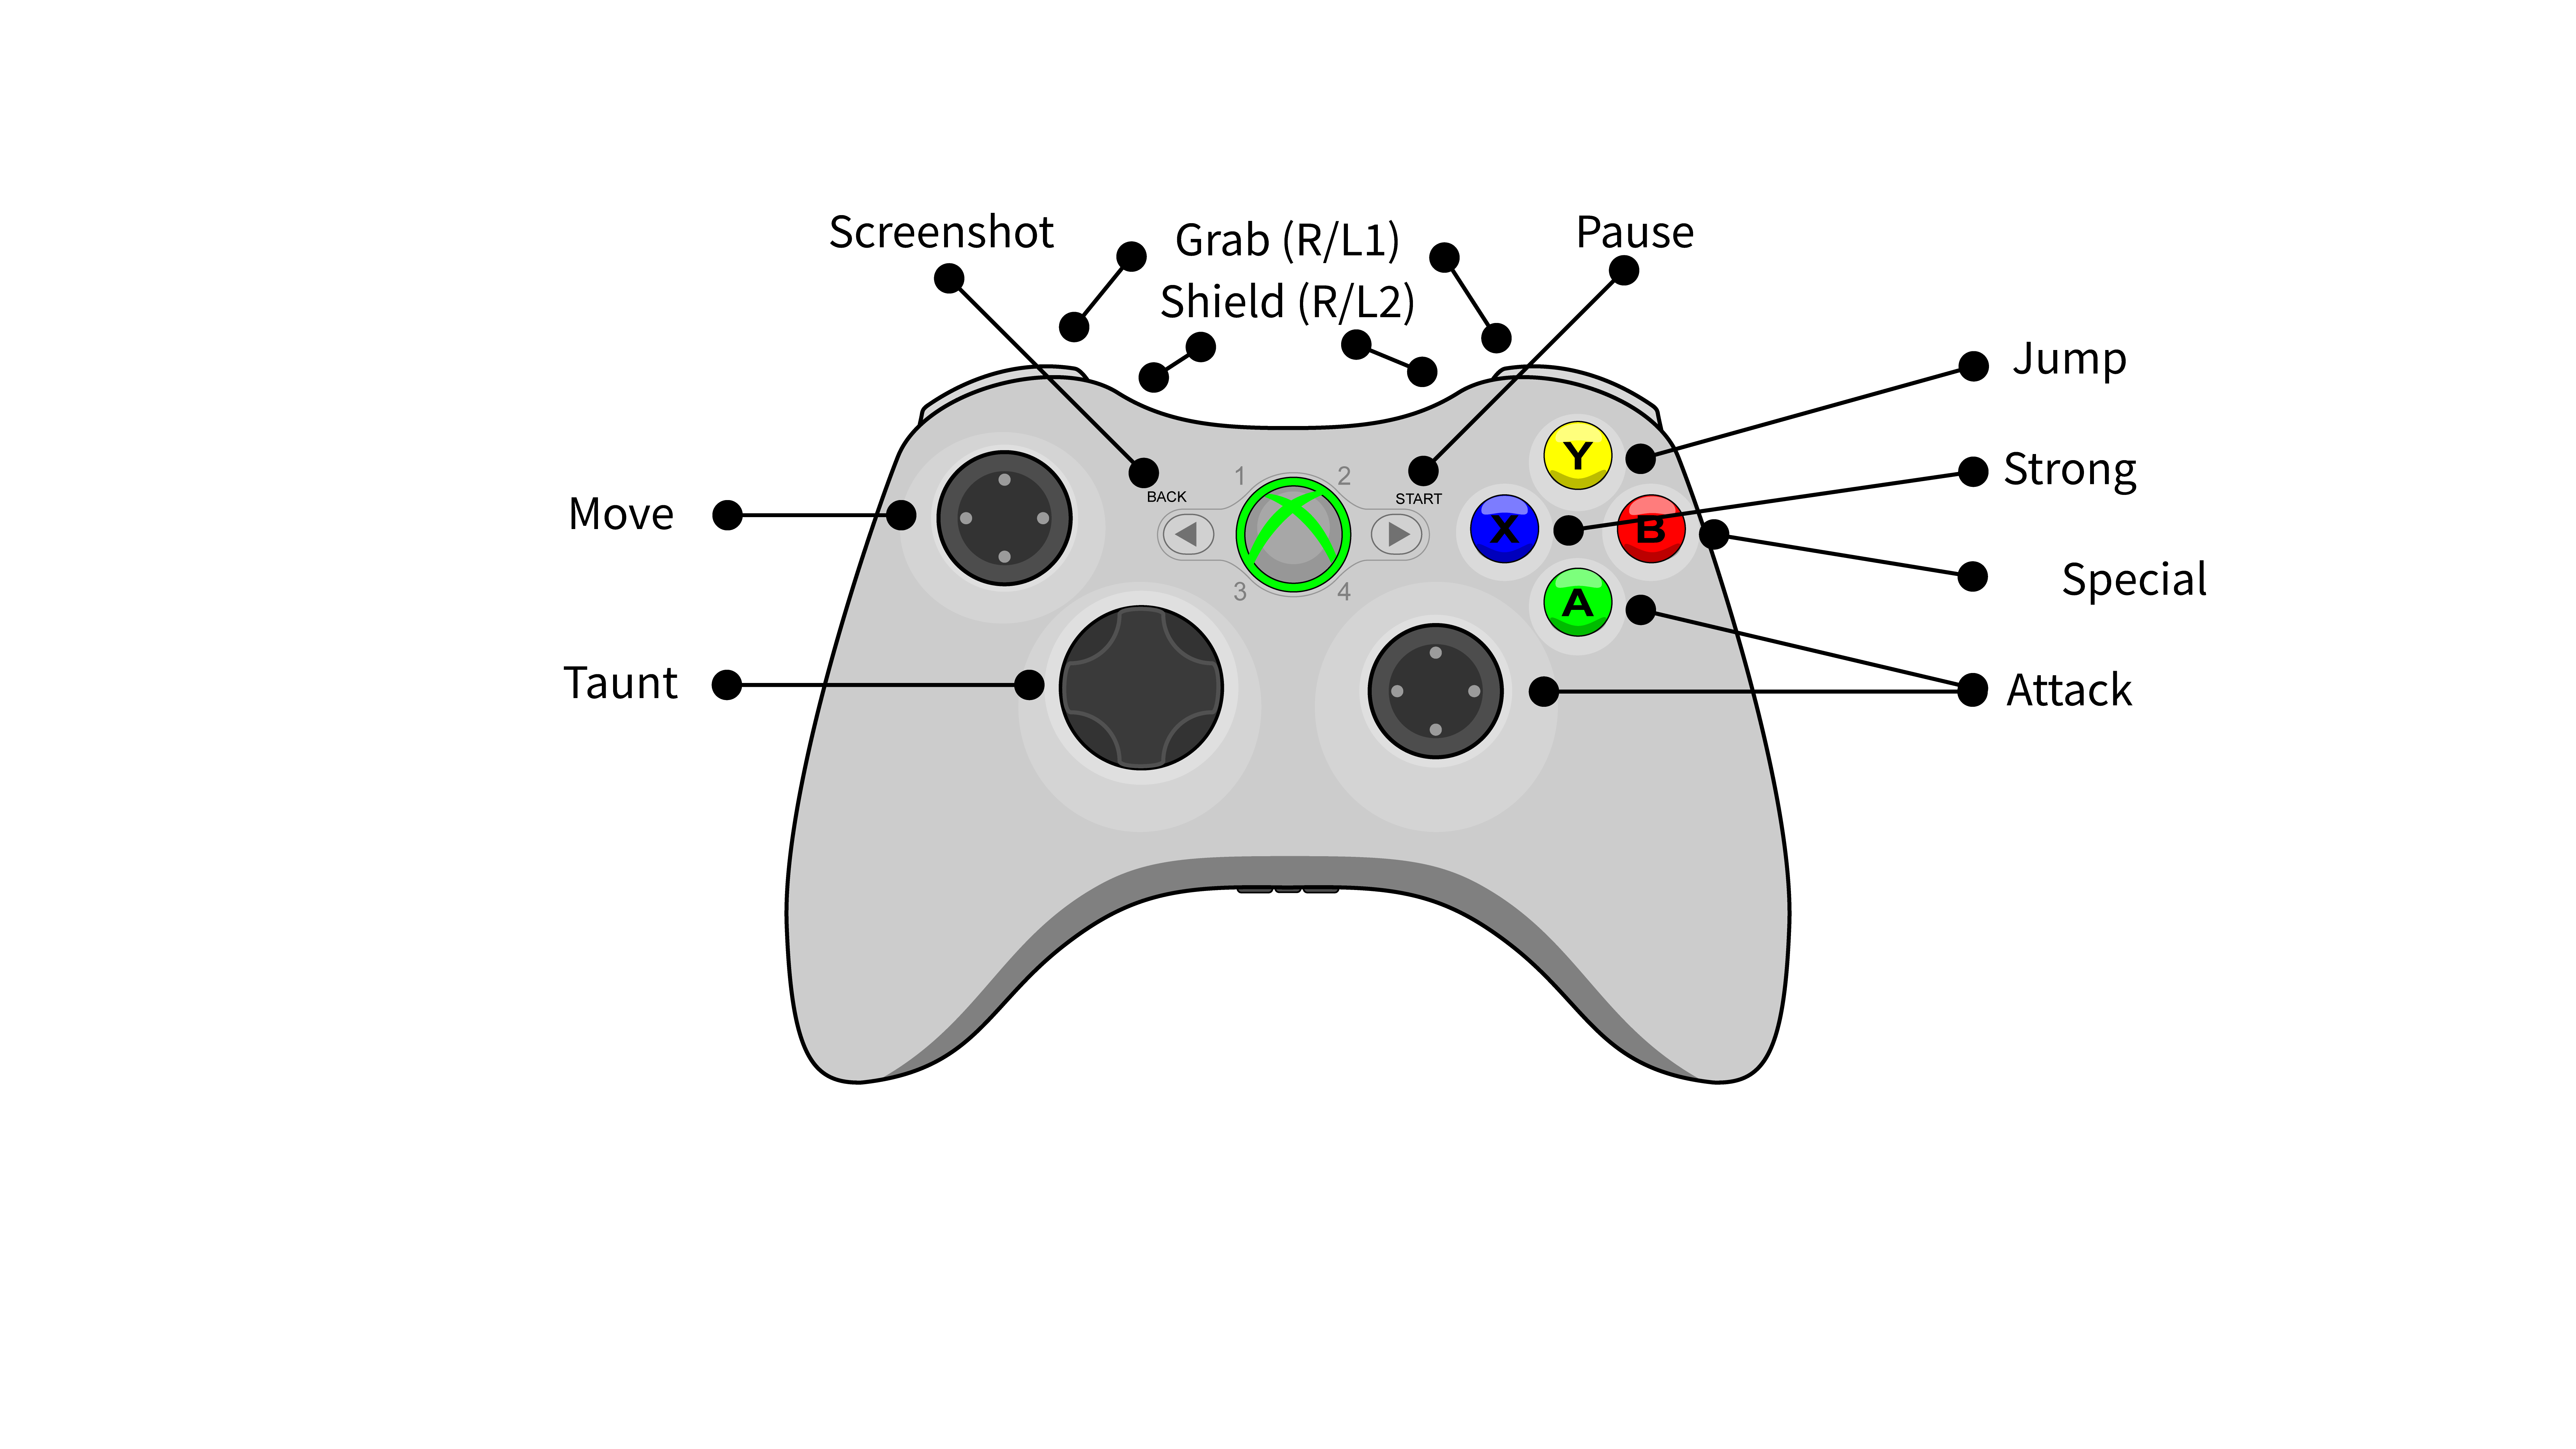
\includegraphics[width=.8\linewidth]{images/gamepad.png}
    \caption{The default gamepad controls for OpenCombat.}
\end{figure}

\begin{figure}[h!]
    \centering
    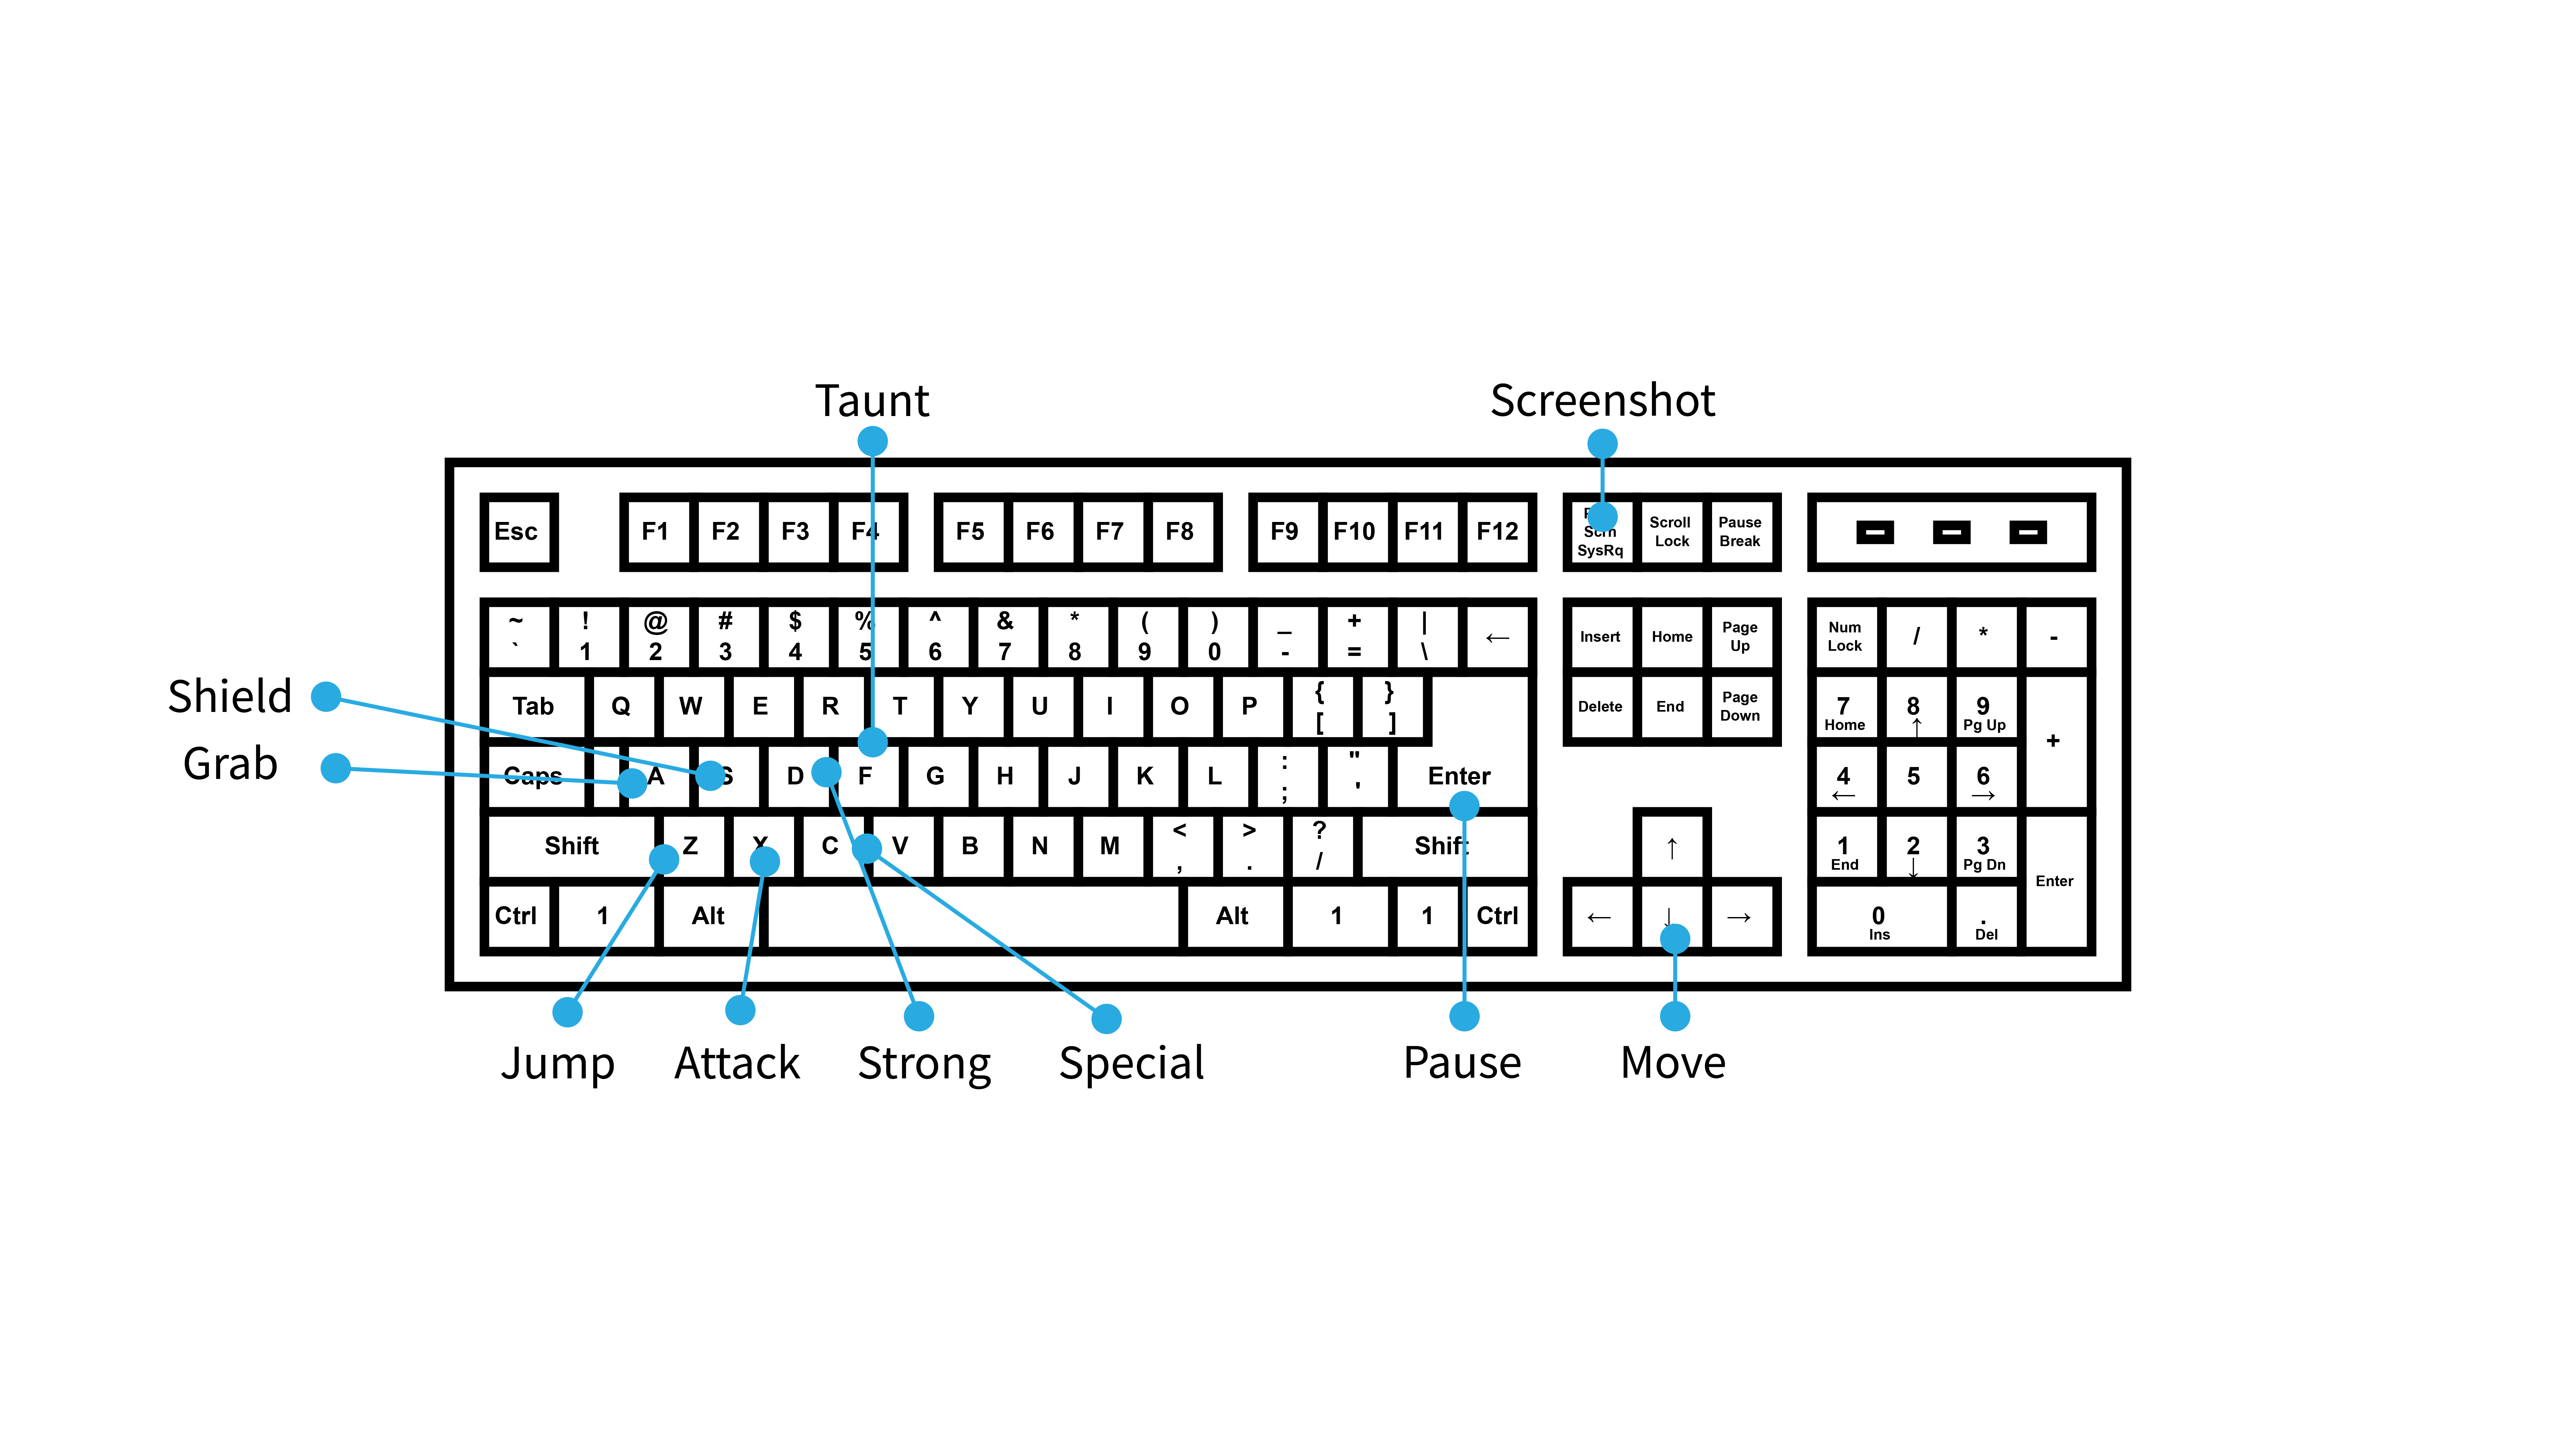
\includegraphics[width=1\linewidth]{images/keyboard.png}
    \caption{The default keyboard controls for OpenCombat.}
\end{figure}

\pagebreak

\section{Directional Arrows Key}

\begin{table}[h!]
    \centering
    \begin{tabular}{| c | c |}
        \hline
        \textbf{Direction} & \textbf{Description} \\
        \hline
        $\rightarrow$ & Away from the player.\\
        \hline
        $\leftarrow$ & Towards the player.\\
        \hline
        $\leftrightarrow$ & Left or right.\\
        \hline
        $\downarrow$ & Down.\\
        \hline
        $\uparrow$ & Up.\\
        \hline
        $\nearrow$ & Up and away from the player.\\
        \hline
        $\searrow$ & Down and away from the player.\\
        \hline
    \end{tabular}
\end{table}

\section{Combat}

\subsection{Overview}

\paragraph{} Similarly to other platform fighting games, OpenCombat matches are fought on stages with varying platform layouts between 2 to 4 players. Players coming from the previously mentioned games will be familiar with the simple button-and-direction execution of actions. These actions include:

\begin{table}[h!]
\centering
\begin{tabular}{ | c | c | c | }
    \hline
    \textbf{Action} & \textbf{Input} & \textbf{Has Aerial Variation?} \\
    \hline
    Jab Attack                                                           & Attack with no direction.            & Yes                   \\
    \hline
    Horizontal Tilt Attack   & Attack + $\leftrightarrow$  & Yes                   \\
    \hline
    Down Tilt Attack                                                     & Attack $\downarrow$                           & Yes                   \\
    \hline
    Up Tilt Attack                                                       & Attack + $\uparrow$          & Yes                   \\
    \hline
    Neutral Special Attack                                               & Special with no direction.           & Yes                   \\
    \hline
    Horizontal Special Attack & Special + $\leftrightarrow$ & Yes                   \\
    \hline
    Down Special Attack                                                  & Special $\downarrow$                          & Yes                   \\
    \hline
    Up Special Attack                                                    & Special + $\uparrow$         & Yes                   \\
    \hline
    Neutral Strong Attack                                                & Strong with no direction             & Yes                   \\
    \hline
    Horizontal Strong Attack                                             & Strong + $\leftrightarrow$  & Yes                   \\
    \hline
    Down Strong Attack                                                   & Strong $\downarrow$                           & Yes                   \\
    \hline
    Up Strong Attack                                                     & Strong + $\uparrow$          & Yes                   \\
    \hline
    Move                                                                 & Left Stick                           & No                    \\
    \hline
    Pause                                                                & Start                                & No                    \\
    \hline
    Screenshot                                                           & Select                               & No                    \\
    \hline
    Shield                                                               & Shield with no direction.            & Yes, performs Dodge   \\
    \hline
    Dodge                                                                & Shield $\downarrow$                           & Yes                   \\
    \hline
    Roll                                                                 & Shield + $\leftrightarrow$  & Yes                   \\
    \hline
    Taunt                                                                & Taunt                                & No \\                  
    \hline
    Jump & Jump & No \\
    \hline
\end{tabular}
\end{table}

\pagebreak

\paragraph{} The OpenCombat experience distinguishes itself from these titles by including new actions and mechanics from 2D traditional fighting games such as:

\begin{itemize}
    \item Stocks and percent are replaced with rounds, matches and stamina (reflected as a percent where 100\% is full health) from traditional fighting games.
    \item Specials and strong attacks, like neutral attacks, have an aerial variation.
    \item Knockback and stun are significantly reduced and do not scale with damage.
\end{itemize}

\paragraph{} Players will utilize all of these actions in order to be the last one remaining. Players can block incoming players' attacks, grab their blocking opponents to catch them off-guard or seize the opportunity to strike if they try to grab them. Players can also take advantage of the unique platform layouts of each stage to put themselves in a position to take the upper hand. Players are eliminated when their stamina reaches 0 or they have been knocked out of the ring.

\paragraph{} The players have complete control over the rules they choose to play with whether they are playing offline or online. Some of these options include:

\begin{itemize}
    \item Rounds
    \item Stamina
    \item Items
    \item Teams
    \item Physics
\end{itemize}

\begin{figure}[h!]
    \centering
    \fbox{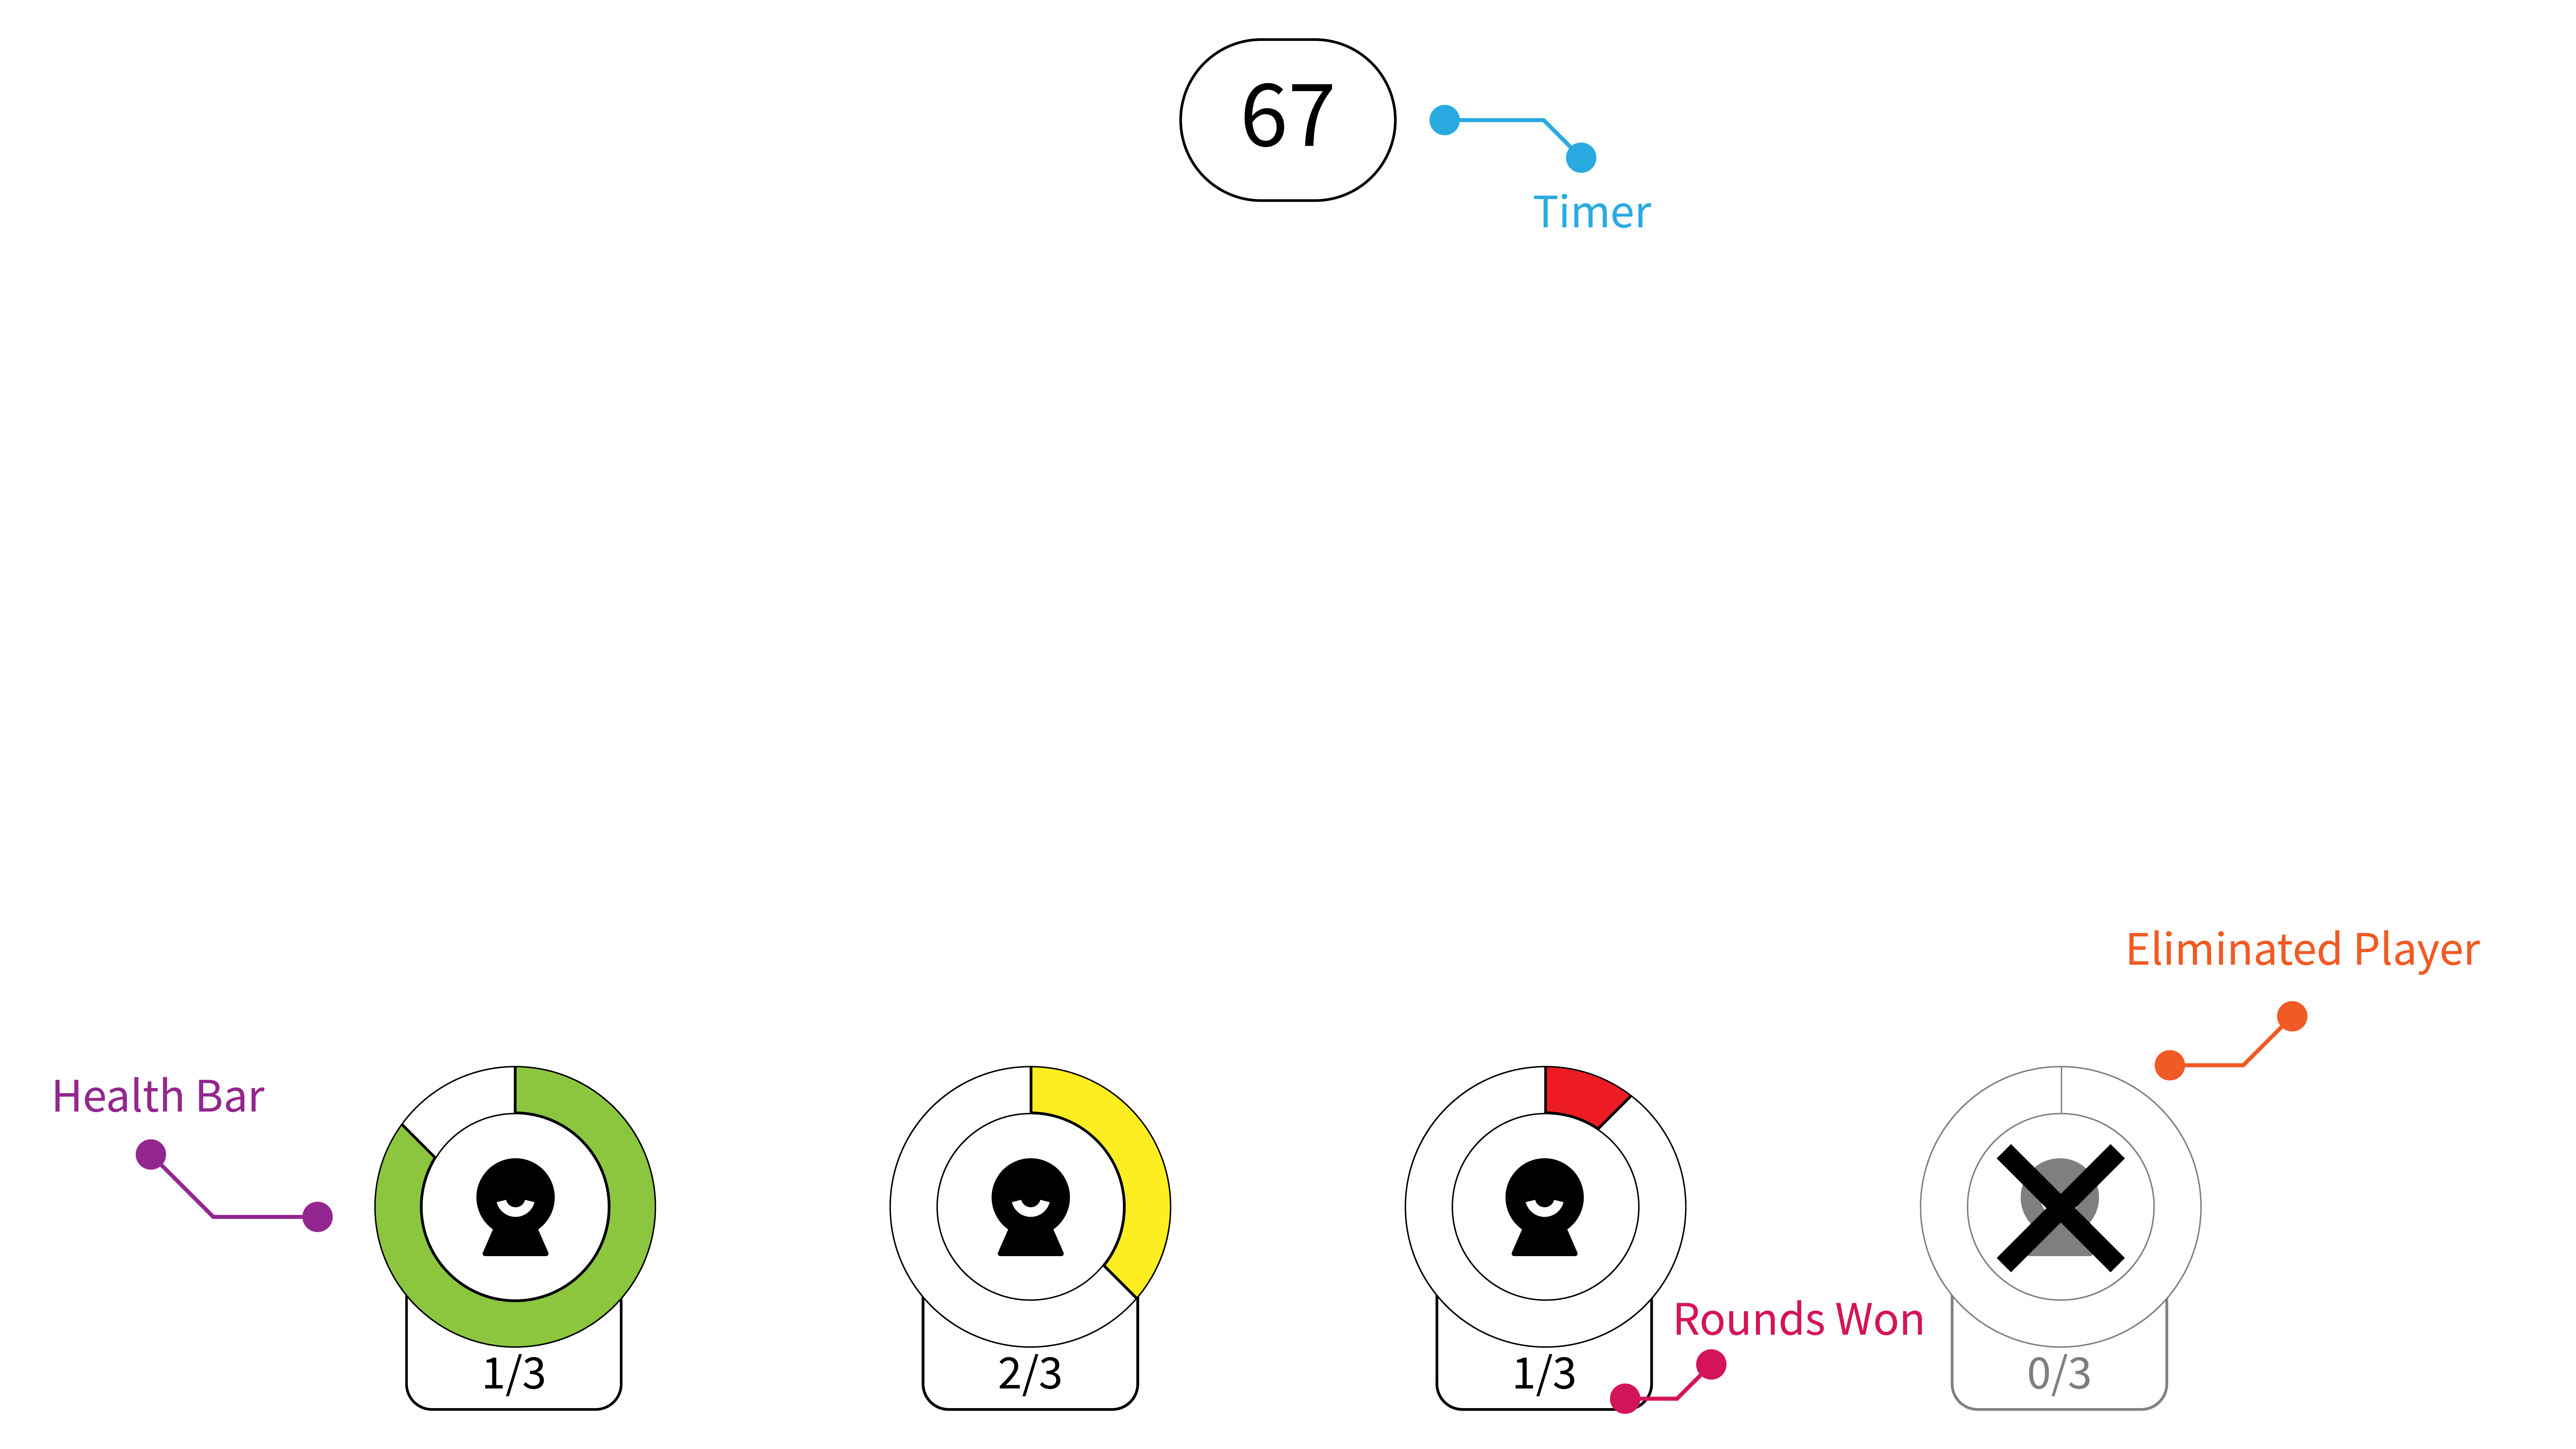
\includegraphics[width=.9\linewidth]{images/combat-ui.png}}
    \caption{The interface of the screen as the players fight.}
\end{figure}

\subsection{Directional Influence}

Directional influence (DI) is the ability for players to slightly change their trajectory by moving while they are in hitstun. This allows players to more easily control where they land after being hit as well as to more easily escape combos. This feature is similar to how it is implemented in Super Smash Bros. Melee and Rivals of Aether; it is designed for more advanced players looking to have more control over their positioning after being hit.

\begin{figure}[h!]
    \centering
    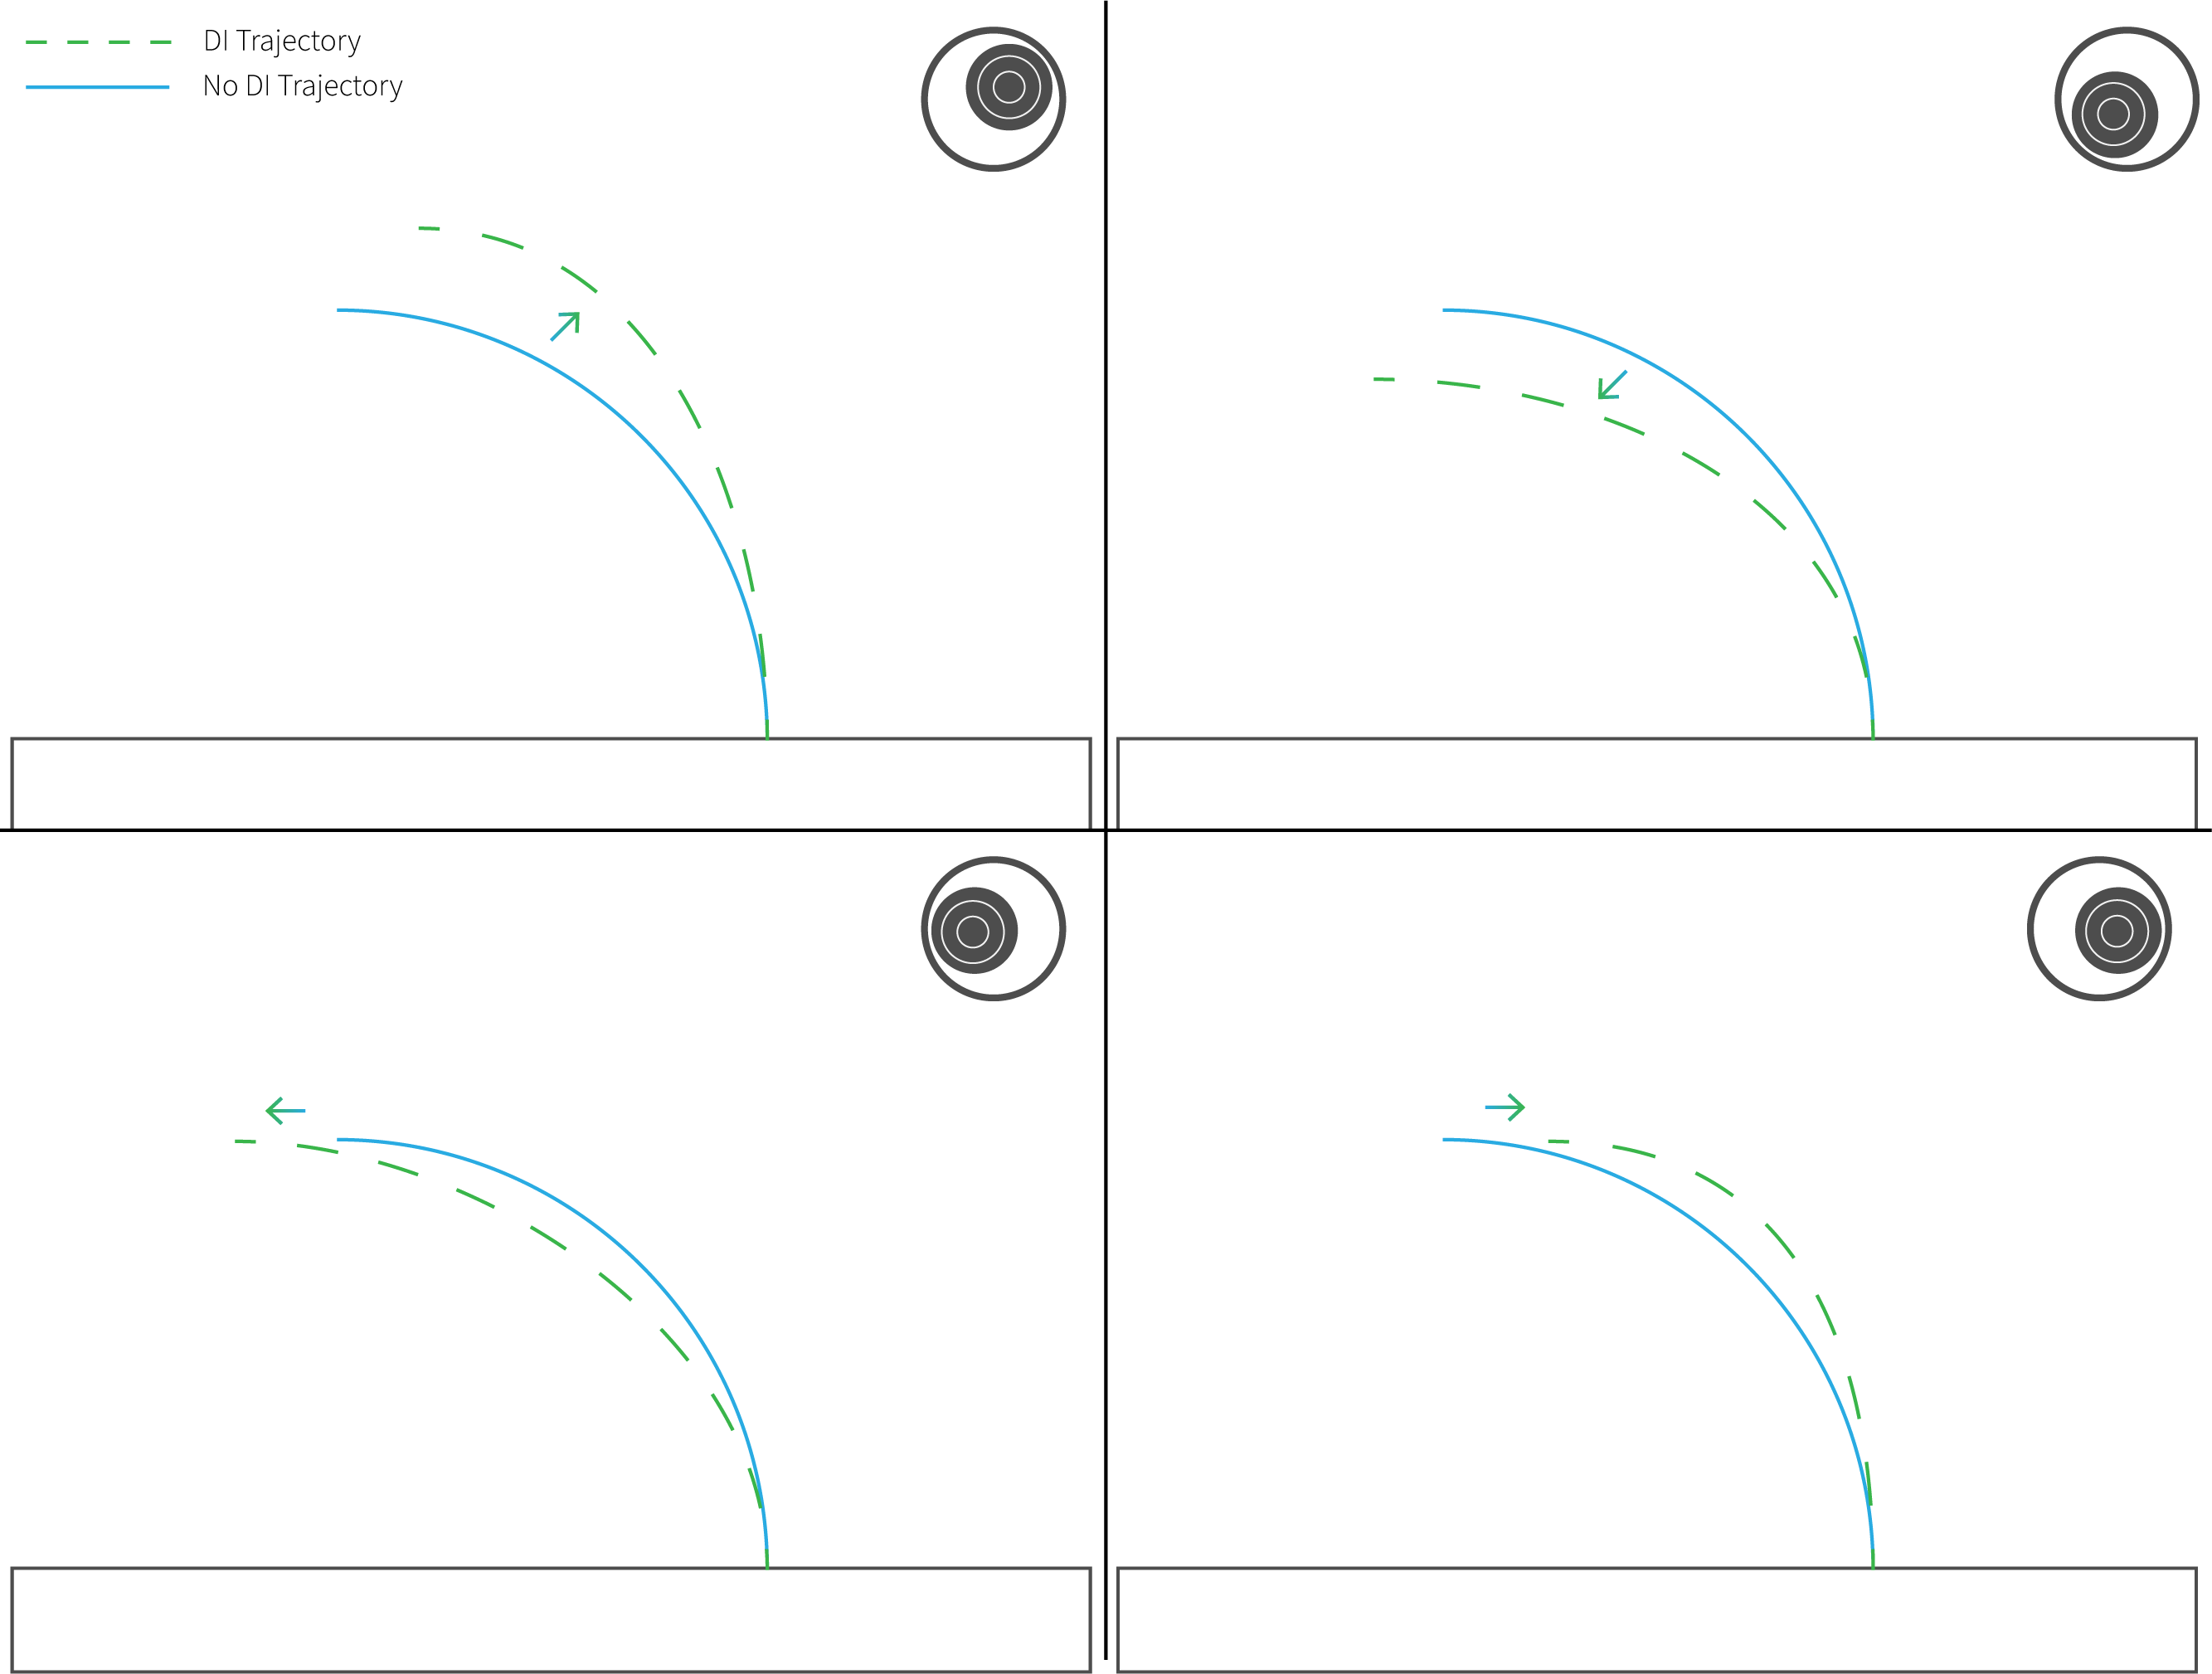
\includegraphics[width=0.8\linewidth]{images/directional-influence.png}
    \caption{By holding directional inputs, players can control their trajectory.}
\end{figure}

\pagebreak

\subsection{Items}

\paragraph{} The audience of a match can throw items into the arena for combatants to use. The audience is usually tame and only throws items into the ring if they have a reason.

\subsubsection{Concessions}

\begin{description}
    \item[Spawn Condition] Combatants have not attacked each other for a while, boring the audience.
    \item[Description] Various empty food containers and other trash that the audience threw into the arena.
    \item[Momentum] Fast
    \item[Distance] Long
    \item[Damage and Effect] 1\% - 2\% on impact.
    \item[Knockback Direction] $\rightarrow$
\end{description}

\noindent\hrulefill

\subsubsection{Underwear}

\begin{description}
    \item[Spawn Condition] One or more combatants is able to successfully finish a taunt.
    \item[Description] Sweaty white boxers, briefs, bras and panties with big red hearts all over them.
    \item[Momentum] Slow
    \item[Distance] Short
    \item[Damage and Effect] 1\% -2\% every .5 seconds the player is within pickup range.
    \item[Knockback Direction] N/A
\end{description}

\noindent\hrulefill

\subsubsection{Confetti F-Bombs}

\begin{description}
    \item[Spawn Condition] When one of the combatants in a match with 3 or more is eliminated.
    \item[Description] Bombs containing confetti shaped like the letter F. They explode upon impact.
    \item[Momentum] Fast
    \item[Distance] Long
    \item[Damage and Effect] 10\% - 25\% based on the player's proximity to the center of the explosion.
    \item[Knockback Direction] $\nearrow$
\end{description}

\noindent\hrulefill

\subsubsection{Headphones}

\begin{description}
    \item[Spawn Condition] The start of the round after a Berserker lost.
    \item[Description] An over-ear pair of headphones that play a rage-inducing voice line.
    \item[Momentum] N/A
    \item[Distance] N/A
    \item[Damage and Effect] Player's movement and damage output is increased by 25\%.
    \item[Knockback Direction] N/A
\end{description}

\paragraph{Voice Lines}

\begin{itemize}
    \item It's pronounced "jif."
    \item Your favorite anime is trash.
    \item Pineapple doesn't belong on pizza.
    \item Always put the ketchup on top of your fries.
    \item Pour the milk in the bowl before you add the cereal.
    \item Water is not wet.
    \item Hot dogs are sandwiches.
    \item You want to listen to my mixtape?
    \item I brush my teeth without wetting the bristles.
\end{itemize}

\noindent\hrulefill

\subsubsection{Tome}

\begin{description}
    \item[Spawn Condition] The start of the round after a Mage lost.
    \item[Description] A thick and heavy academic text book.
    \item[Momentum] Medium
    \item[Distance] Medium
    \item[Damage and Effect] 10\% - 15\% on impact.
    \item[Knockback Direction] $\nearrow$
\end{description}

\noindent\hrulefill

\subsubsection{Ale}

\begin{description}
    \item[Spawn Condition] The start of the round after a Sailor lost.
    \item[Description] A bottle of bright gold, frothy ale that gives combatants more confidence but less grace.
    \item[Momentum] Fast
    \item[Distance] Long
    \item[Damage and Effect] Reduces movement speed by 25\% but increases damage by 50\%. 4\% - 5\% on impact.
    \item[Knockback Direction] $\rightarrow$
\end{description}

\noindent\hrulefill

\subsubsection{Treats}

\begin{description}
    \item[Spawn Condition] The start of the round after a Druid lost.
    \item[Description] An animal biscuit that can be consumed to restore health.
    \item[Momentum] N/A
    \item[Distance] N/A
    \item[Damage and Effect] Restores 5\% of damage taken.
    \item[Knockback Direction] N/A
\end{description}

\noindent\hrulefill

\subsubsection{Battleaxe}

\begin{description}
    \item[Spawn Condition] The start of the round after a Heavy lost.
    \item[Description] A large metal battleaxe with dents, scratches and bloodstains.
    \item[Momentum] Slow
    \item[Distance] Long
    \item[Damage and Effect] 20\% - 25\% on impact. This item can only be picked up by large characters.
    \item[Knockback Direction] $\searrow$
\end{description}

\noindent\hrulefill

\subsubsection{Zen Grass}

\begin{description}
    \item[Spawn Condition] The start of the round after a Monk lost.
    \item[Description] A mysterious plant from the high mountains that can be consumed for enjoyment.
    \item[Momentum] N/A
    \item[Distance] N/A
    \item[Damage and Effect] Player's movement and damage output is increased by 25\%.
    \item[Knockback Direction] N/A
\end{description}

\noindent\hrulefill

\section{Matchmaking and Player Profiles}

\paragraph{} Players can fight it out online in private matches or by using online matchmatching. When players first start the game, they create a local profile that is used to keep track of their wins, losses and other in-game data. These profiles can be synced to an optional online account so players can simply log in and have access to their information from anywhere. At any point, the player can choose to reset their progress and have their data deleted.

\section{Community Organizing Tool and Community Level}

\paragraph{} The community organizing tool is designed for every type of user from the college sophomore looking to have some friends over to the tournament organizer preparing for a large event. Organizers can post information about their event, track attendance, setup brackets and quickly communicate with all parties involved to coordinate without needing social media or external services. The average player will find the community organizing tool to be a helpful way to plan ahead for social gatherings as well as find local events to play at. To encourage players to come together and plan community events, player profiles will have a community level where experience is gained from playing matches at community events, hosting events and being commended by your fellow players for sportsmanship, teamwork, positivity, etc.

\paragraph{} The community as a whole also shares an experience pool called the community level. Separate from each player's individual level, the community level is a reflection of the player bases' activities; the community earns experience by playing matches, attending real-world events and donating to the studio. When updates are released, the community will have to reach certain experience point goals in order to unlock the content for everyone. For example, new costumes for characters may require the community level to be $\frac{1}{3}$ of the way to the next level while a new playable class will require the community to reach the next level. The community level will always be capped to one additional level per update.

\begin{figure}[h!]
    \centering
    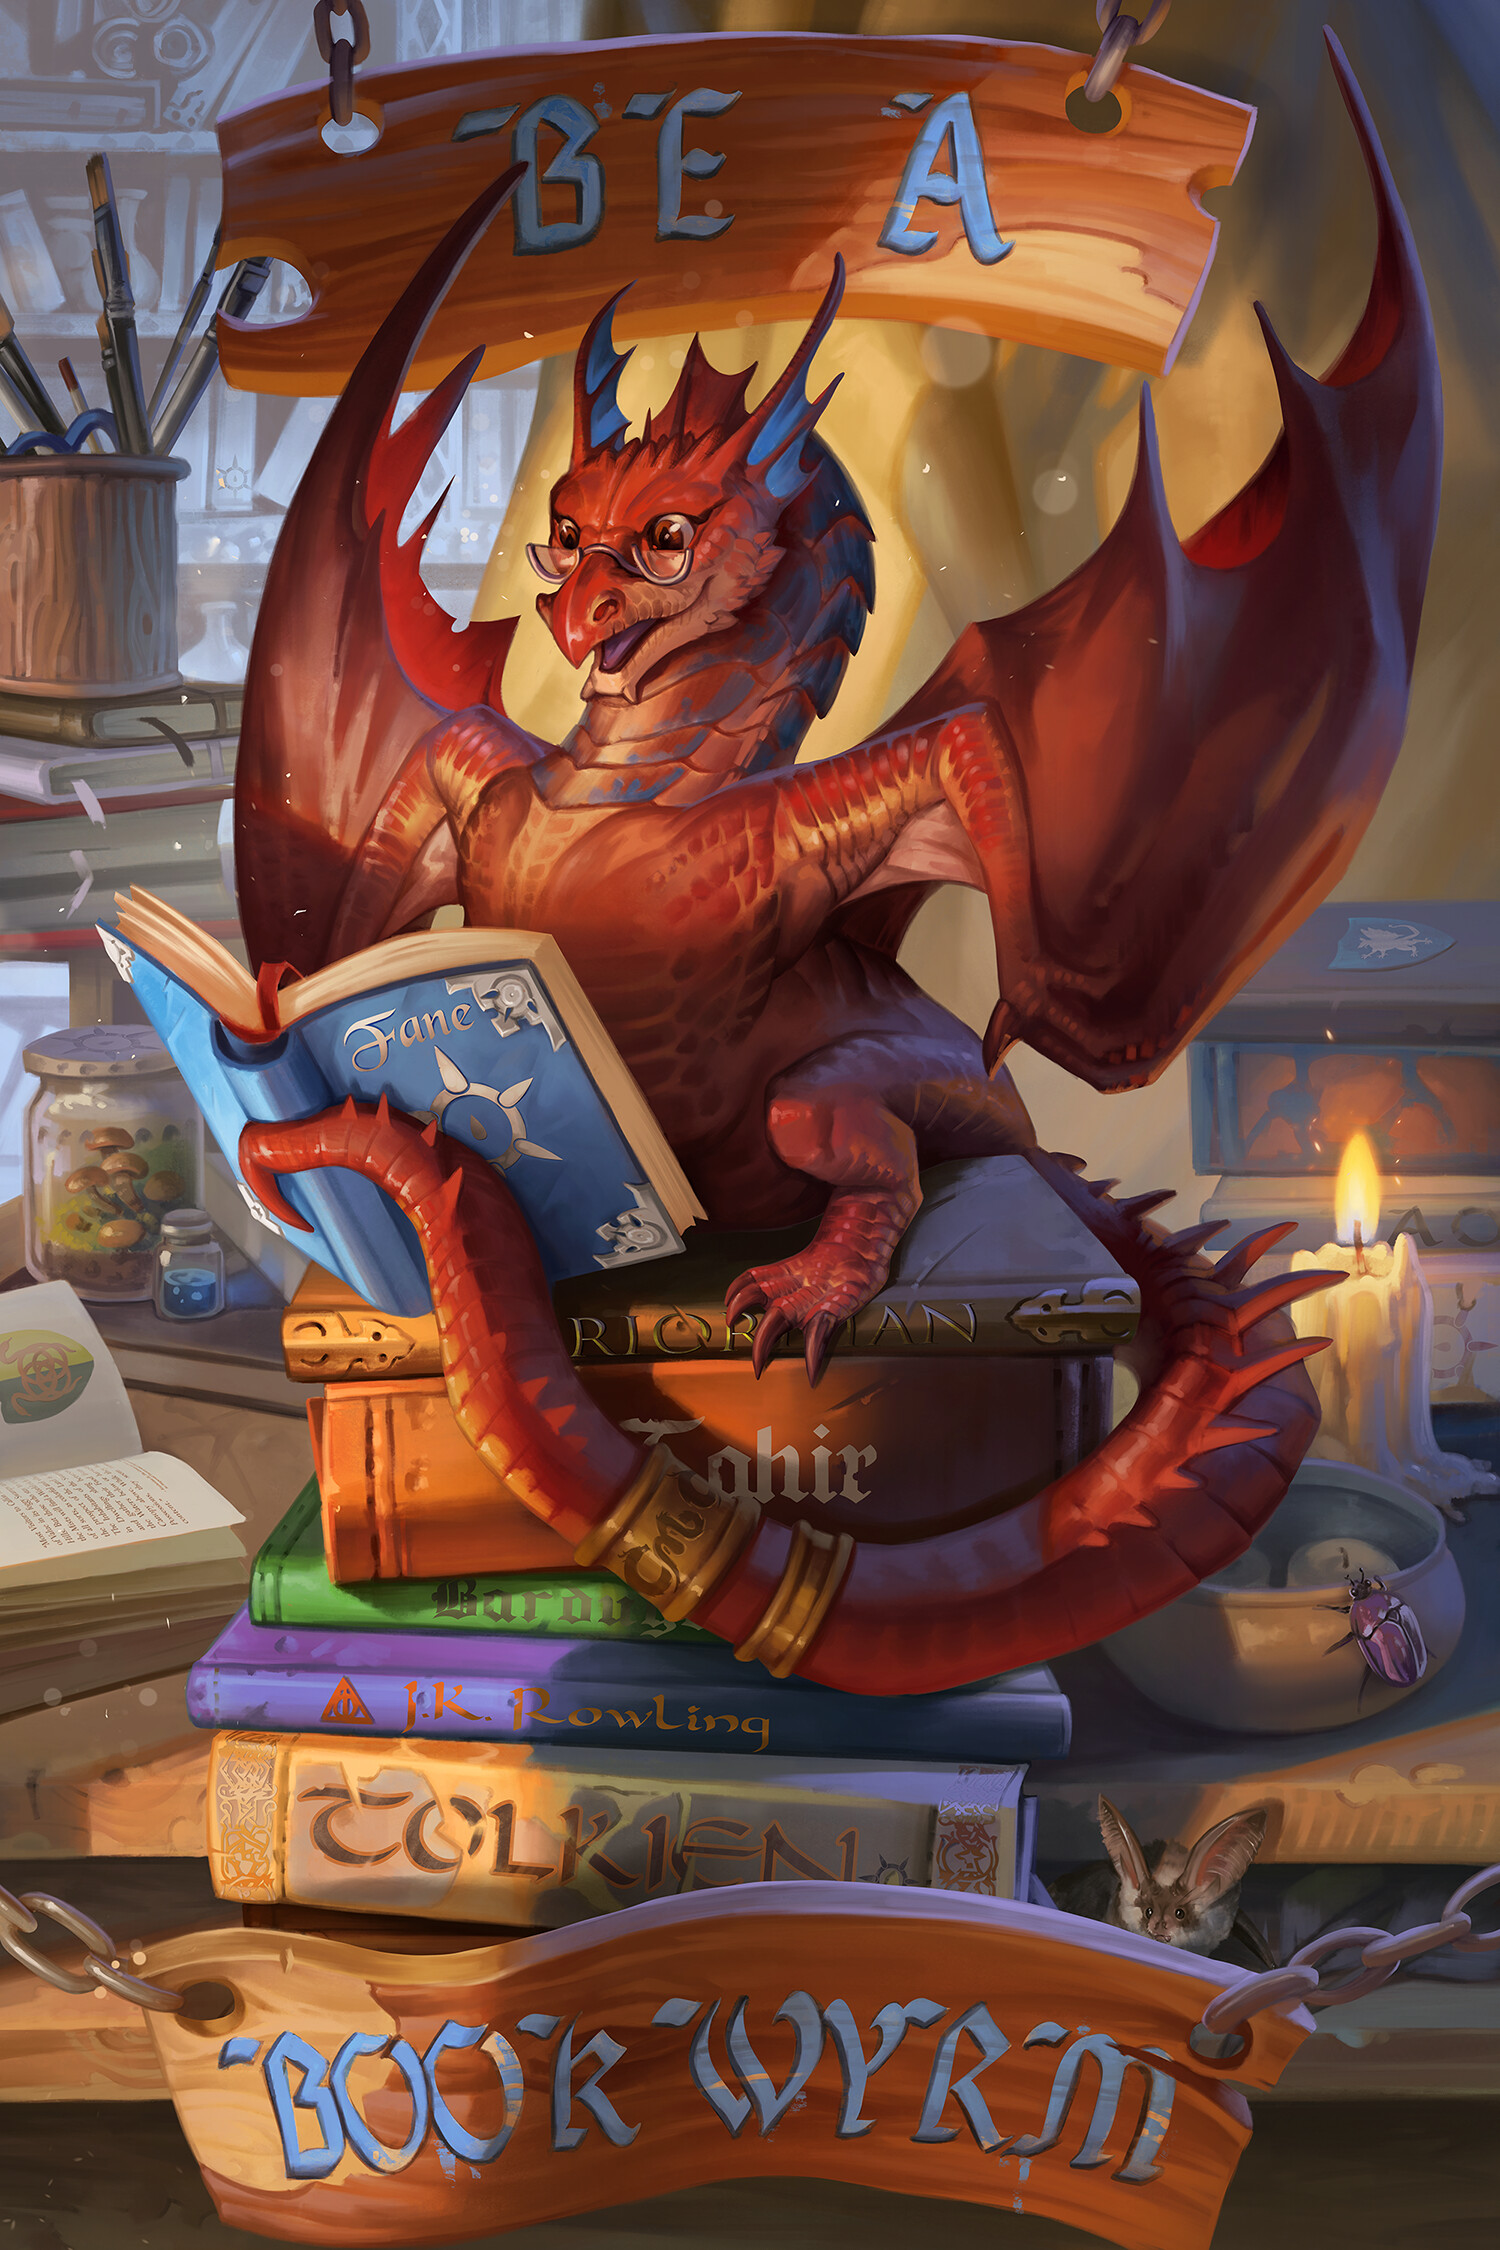
\includegraphics[width=0.35\linewidth]{images/characters-dragon.jpg}
    \caption{Book Wyrm by Milica \v{C}elikovi\'{c}.\nocite{celikovic_book_2019}}
\end{figure}

\pagebreak

\begin{figure}[h!]
    \centering
    \fbox{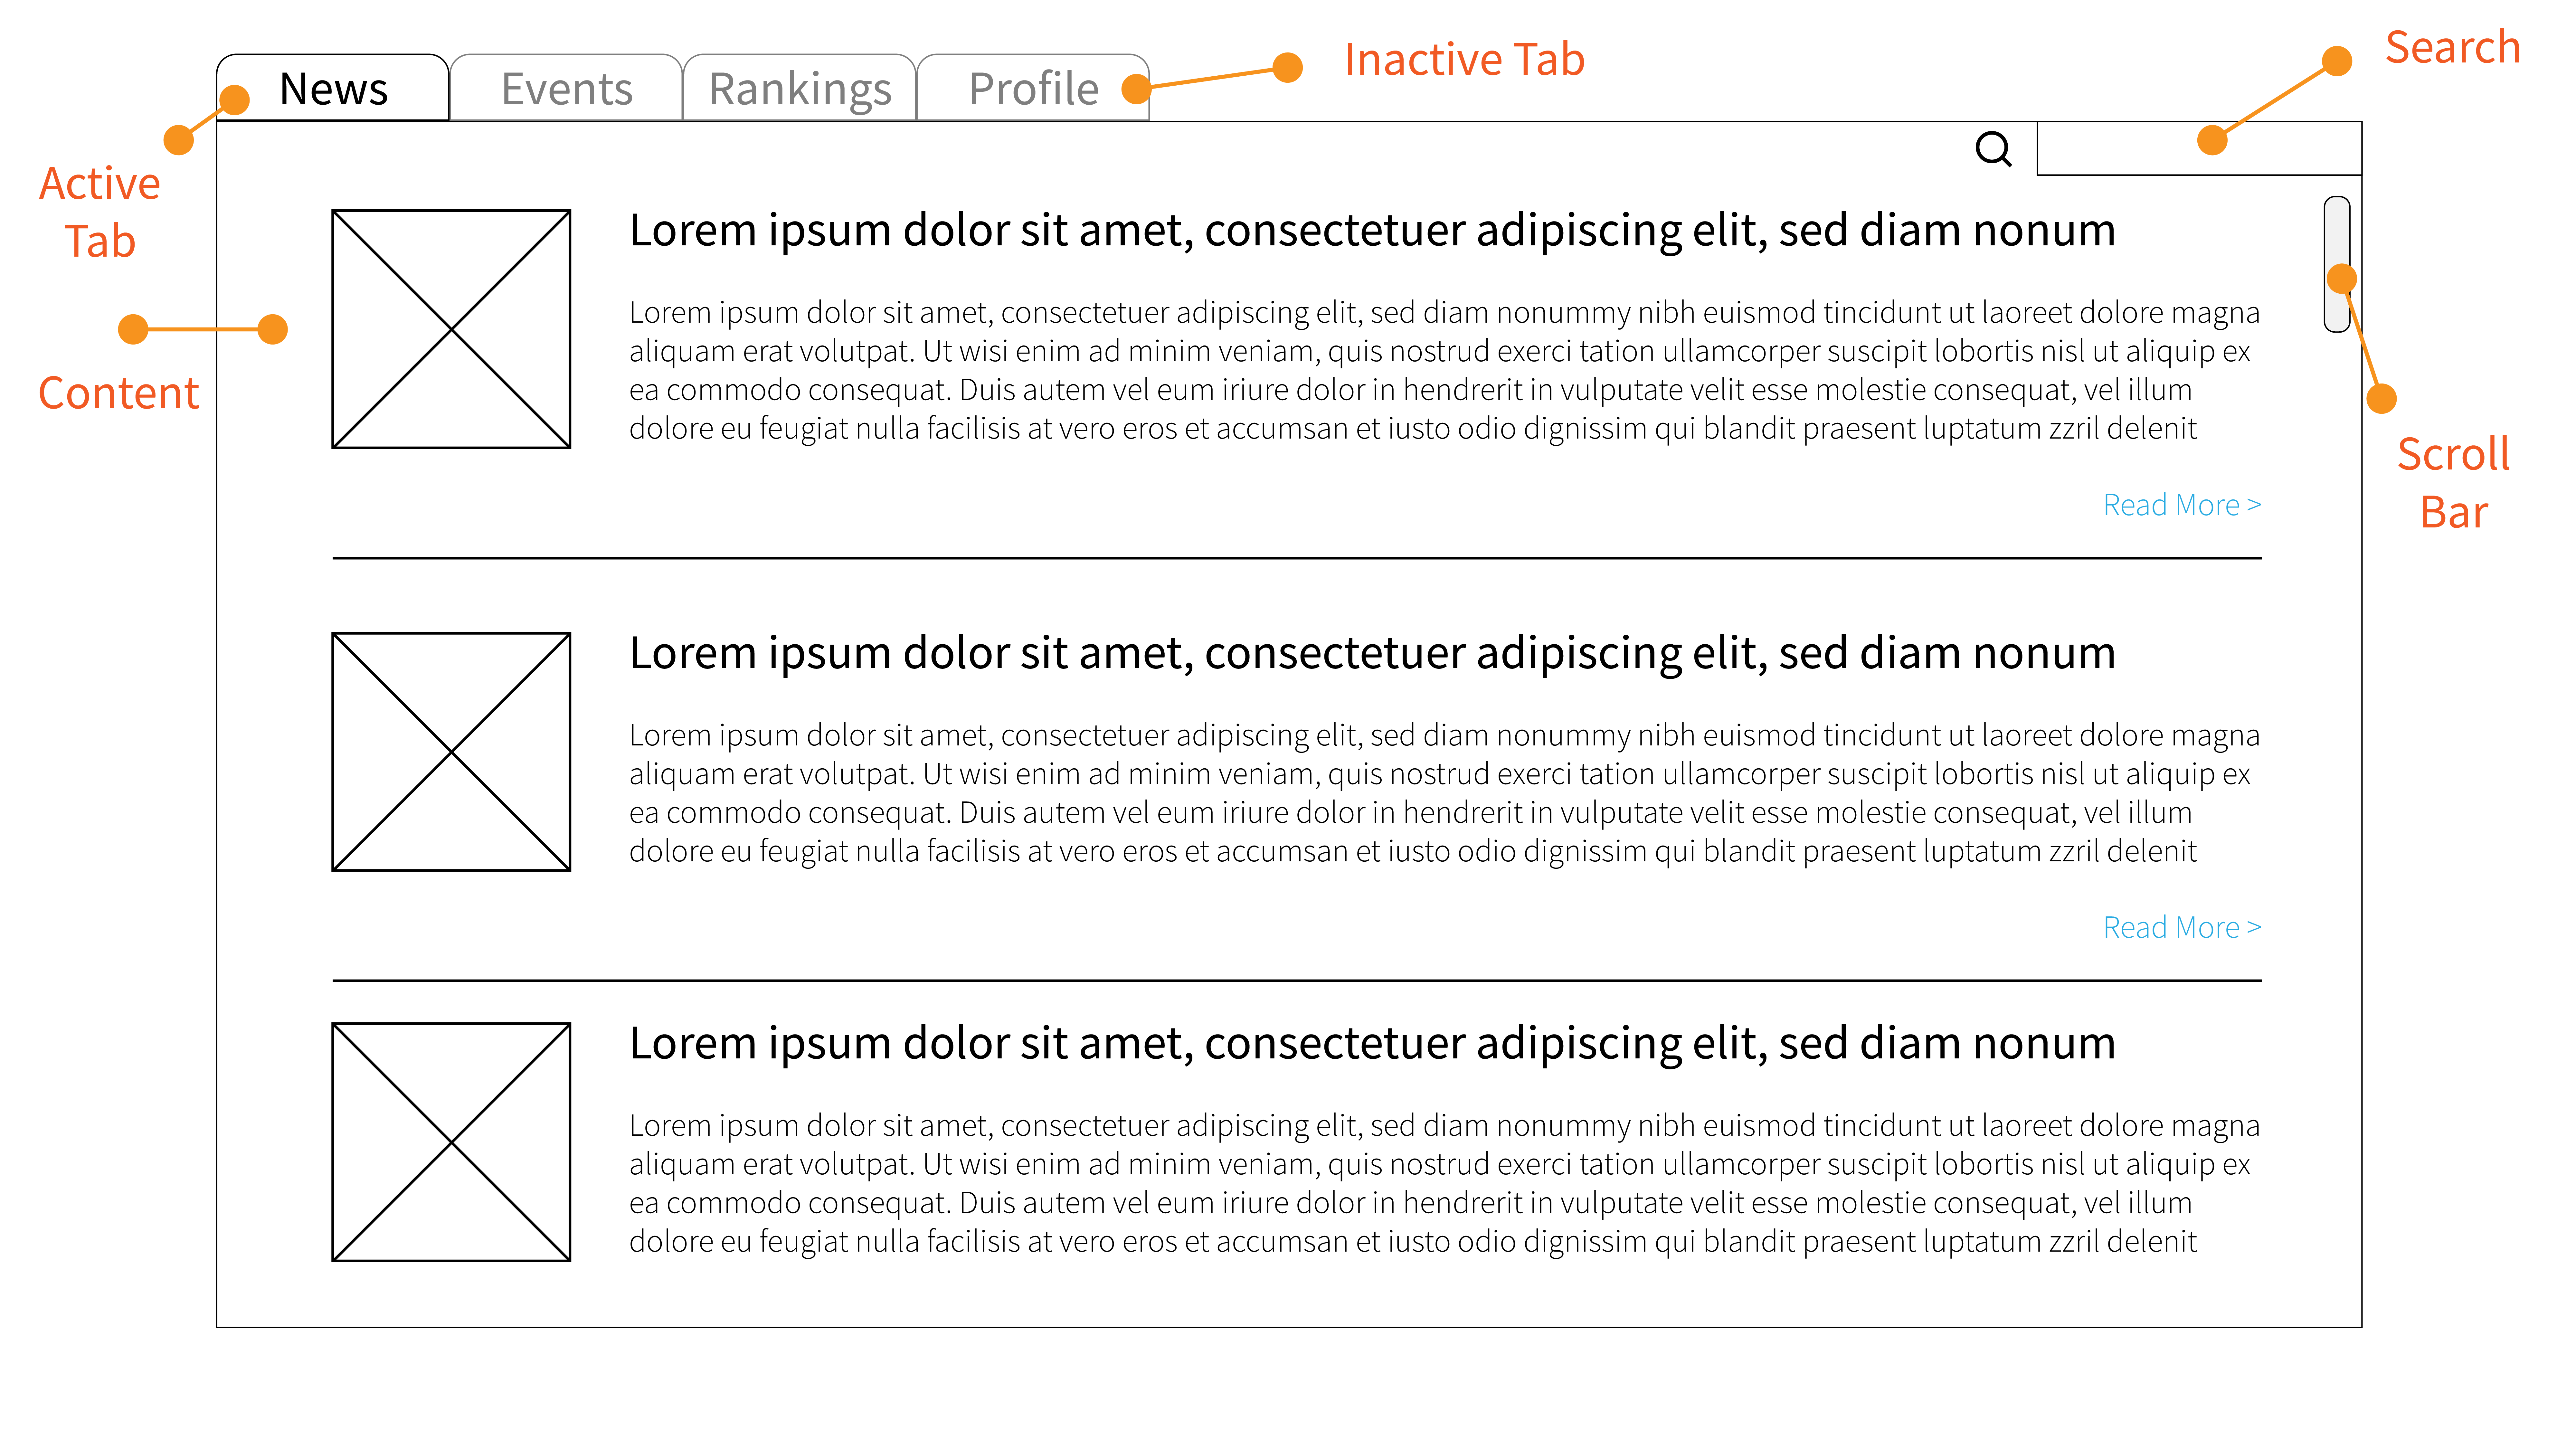
\includegraphics[width=1\linewidth]{images/community-tool.png}}
    \caption{The community organizing tool in the game.}
\end{figure}

\begin{figure}[h!]
    \centering
    \fbox{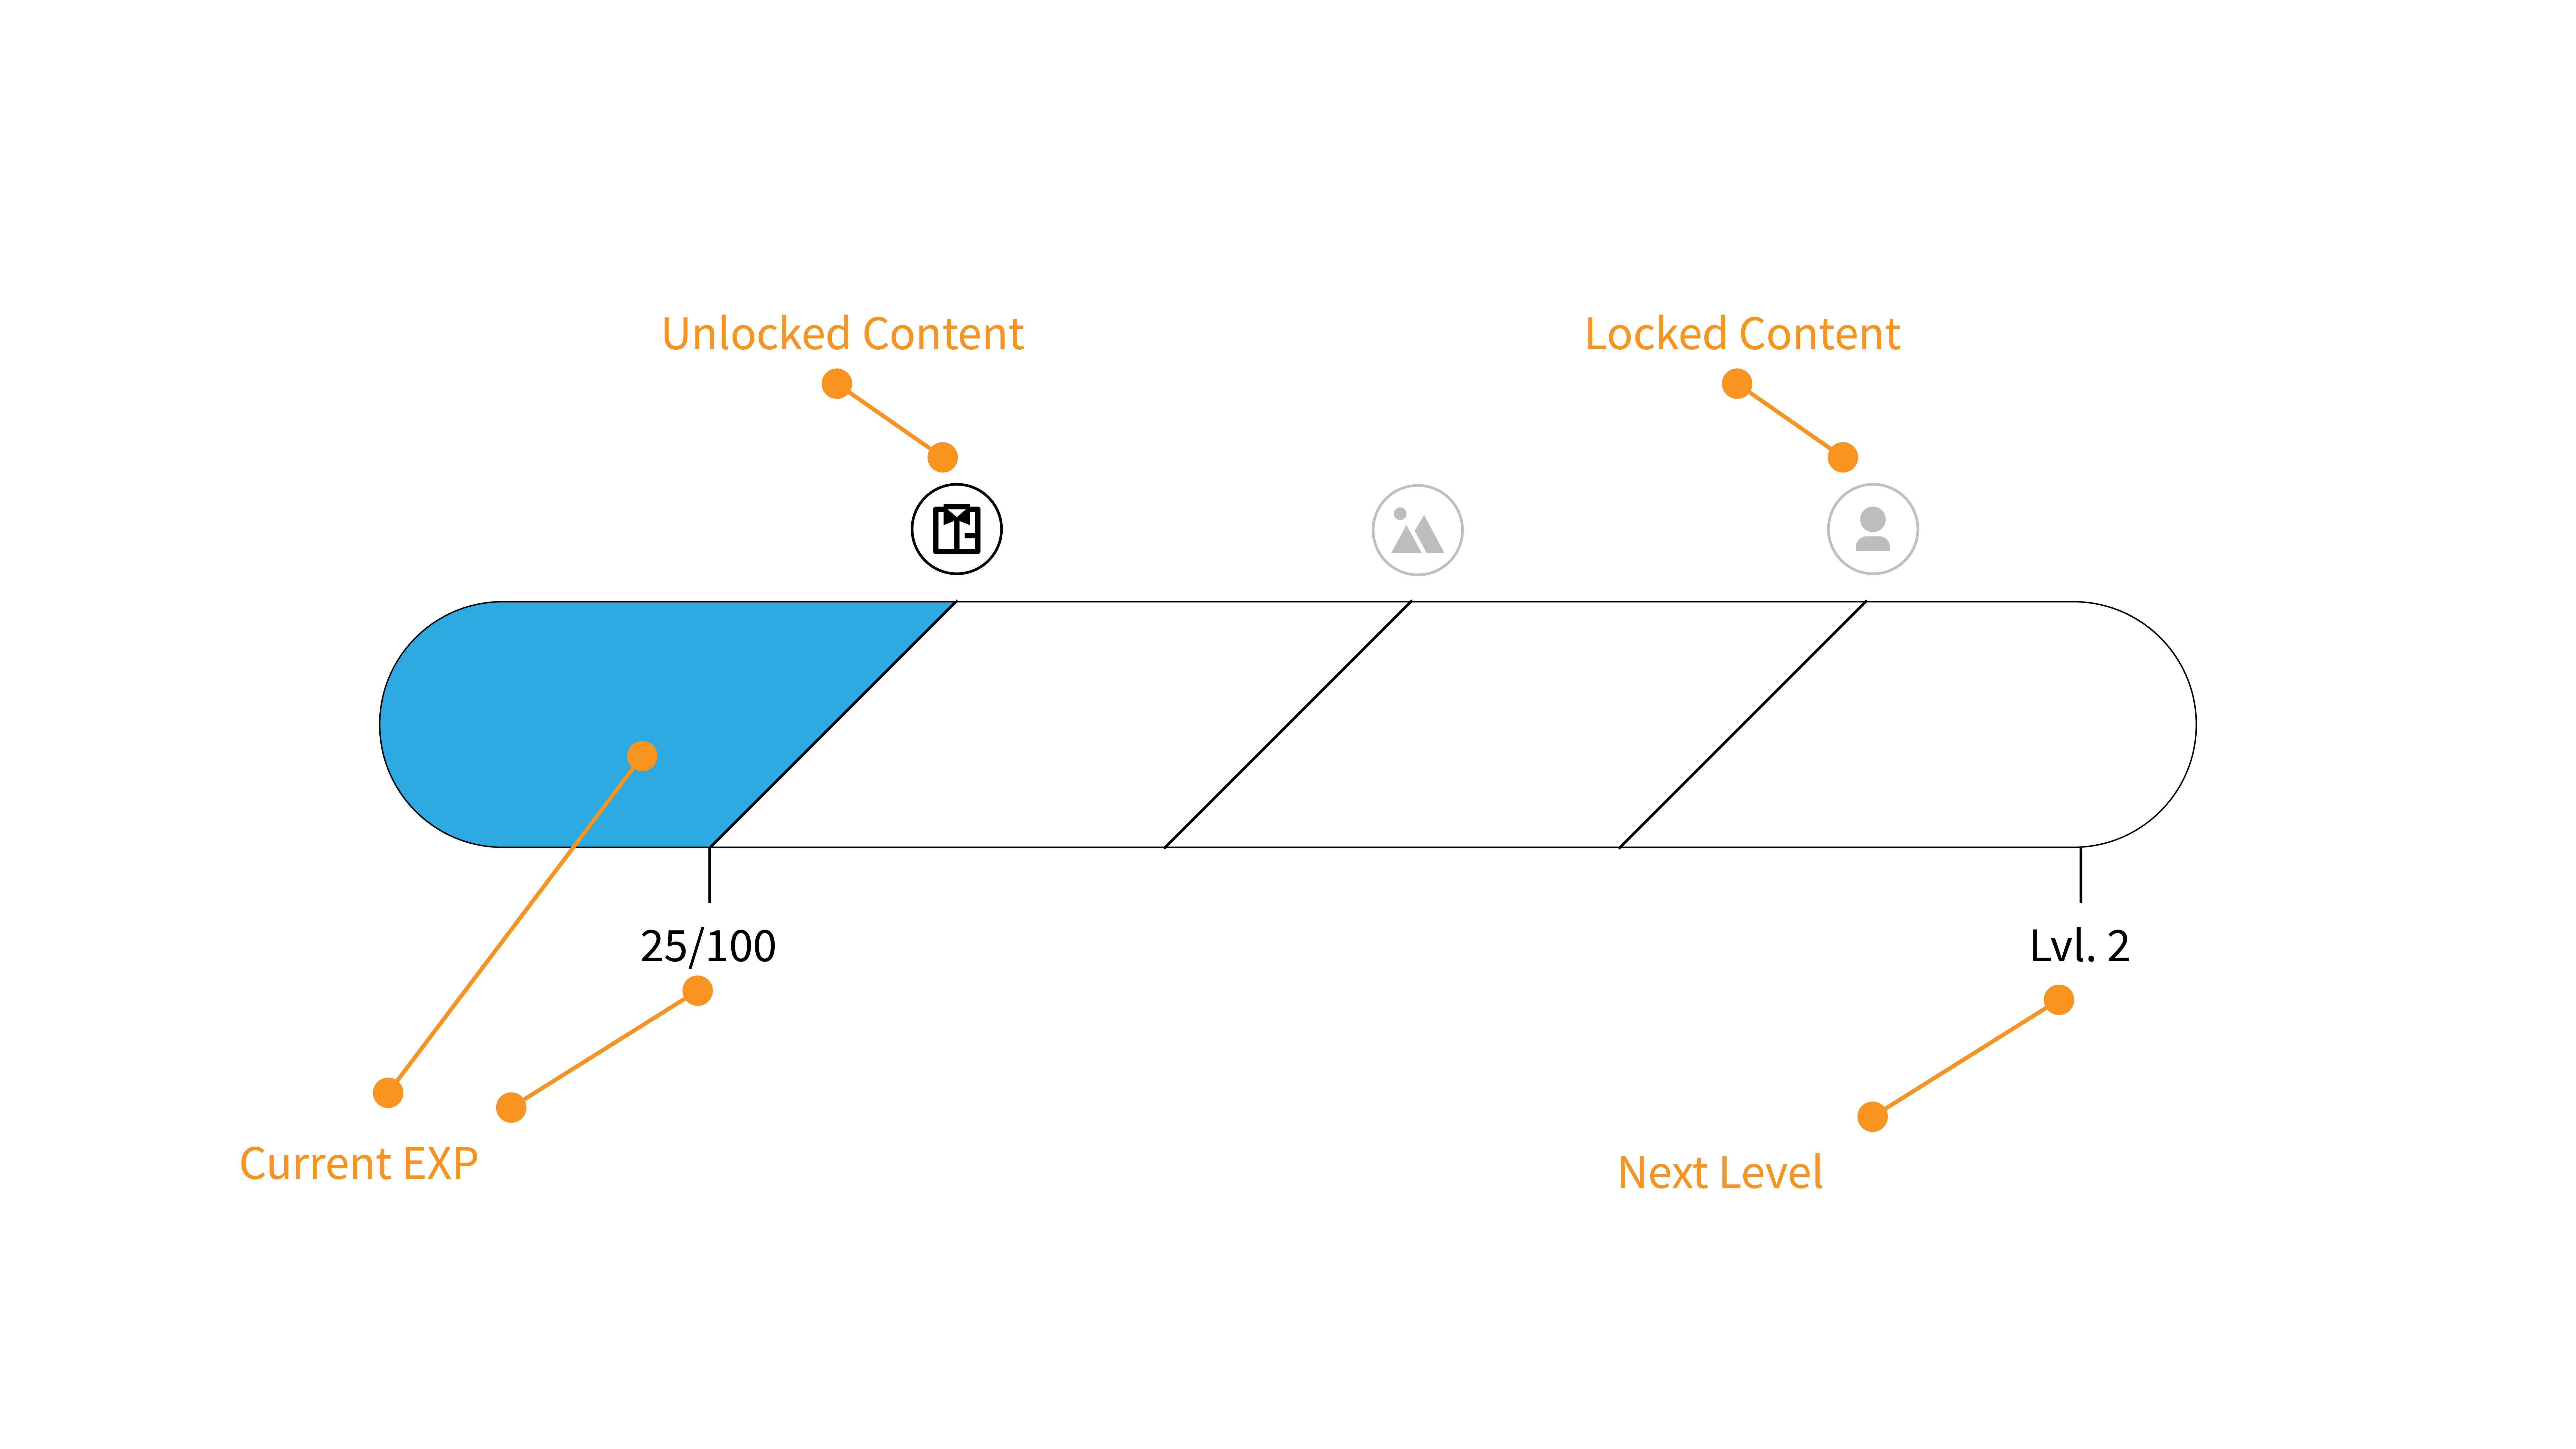
\includegraphics[width=1\linewidth]{images/community-level.png}}
    \caption{The community organizing tool in the game.}
\end{figure}

\pagebreak

\section{Custom Combatants}

\paragraph{} Players can create their own custom combatant based on 1 of 6 classes. They can customize their physical appearance, clothing and biographical information. Each of these classes come with their own movesets, strengths and weaknesses.

\subsection{Playable Classes}

\subsubsection{Mage}

\begin{description}
    \item[Archetype] Zoner
    \item[Body Size] Medium
    \item[Number of Jumps] 2
    \item[Ground Speed] Average
    \item[Aerial Speed] Average    
\end{description}

\paragraph{Description} Combatants who can wield the arcane arts use it to control the space around them and keep their opponents away. Although these fighters move on the ground at a moderate speed, they are able to better control their aerial movement despite their average weight. While they are great at keeping slower opponents away, they are weak against opponents that can rush and attack them.

\begin{table}[h!]
    \centering
    \begin{tabular}{| c | c | c | c | c | c | c |}
        \hline
        \textbf{Attack} & \textbf{Damage} & \textbf{Speed} & \textbf{Range} & \textbf{Launch/Hitstun} & \textbf{Super Armor} & \textbf{Knockback} \\
        \hline
        Jab & 1\% - 2\% & Very Fast & Medium & N/A & No & N/A \\
        \hline
        Horizontal Tilt & 5\% - 7\% & Fast & Long & Short & No & $\rightarrow$ \\
        \hline
        Down Tilt & 4\% - 6\% & Average & Medium & Short & No & $\searrow$ \\
        \hline
        Up Tilt & 4\% - 6\% & Fast & Short & Short & No & $\nearrow$ \\
        \hline
        Neutral Special & 10\% - 12\% & Average & Medium & Average & No & $\rightarrow$ \\
        \hline
        Horizontal Special & 6\% - 7\% & Very Fast & Long & N/A & No & N/A \\
        \hline
        Down Special & 15\% - 17\% & Slow & Short & Long & No & $\rightarrow$ \\
        \hline
        Up Special & 11\% - 12\% & Average & Medium & Average & No & $\nearrow$ \\
        \hline
        Neutral Strong & 15\% - 17\% & Slow & Long & Long & No & $\rightarrow$ \\
        \hline
        Horizontal Strong & 16\% - 18\% & Slow & Long & Long & No & $\nearrow$ \\
        \hline
        Down Strong & 12\% - 13\% & Average & Short & Average & No & $\searrow$ \\
        \hline
        Up Strong & 15\% - 17\% & Fast & Short & Long & No & $\uparrow$ \\
        \hline
        Neutral Aerial Tilt & 6\% - 8\% & Very Fast & Long & Short & No & $\rightarrow$ \\
        \hline
        Horizontal Aerial Tilt & 4\% - 7\% & Very Fast & Long & Short & No & $\rightarrow$ \\
        \hline
        Down Aerial Tilt & 7\% - 8\% & Fast & Average & Average & No & $\downarrow$ \\
        \hline
        Up Aerial Tilt & 8\% - 9\% & Average & Short & Average & No & $\uparrow$ \\
        \hline
        Neutral Aerial Special & 12\% - 13\% & Average & Medium & Average & No & $\rightarrow$ \\
        \hline
        Horizontal Aerial Special & 8\% - 10\% & Very Fast & Long & N/A & No & N/A \\
        \hline
        Down Aerial Special & 18\% - 20\% & Very Slow & Short & Long & No & $\downarrow$ \\
        \hline
        Up Aerial Special & 9\% - 12\% & Fast & Short & Short & No & $\nearrow$ \\
        \hline
        Neutral Aerial Strong & 12\% - 13\% & Slow & Average & Average & No & $\rightarrow$ \\
        \hline
        Horizontal Aerial Strong & 14\% - 16\% & Very Slow & Long & Long & No & $\rightarrow$ \\
        \hline
        Down Aerial Strong & 11\% - 12\% & Slow & Short & Average & No & $\searrow$ \\
        \hline
        Up Aerial Strong & 14\% - 15\% & Very Fast & Short & Long & No & $\uparrow$ \\
        \hline
    \end{tabular}
\end{table}

\pagebreak

\subsubsection{Sailor}

\begin{description}
    \item[Archetype] Grappler
    \item[Body Size] Medium
    \item[Number of Jumps] 2
    \item[Ground Speed] Average
    \item[Aerial Speed] Average 
\end{description}

\paragraph{Description} From the sea to the shore, sailors are the undisputed masters of the cutlass and hookshot. Their average mobility, power and speed are offset by their ability to pull distant opponents towards them. The sailors' hookshots give them a distinct advantage over range opponents but they can be easily be overwhelmed by faster fighters.

\begin{table}[h!]
    \centering
    \begin{tabular}{| c | c | c | c | c | c | c |}
        \hline
        \textbf{Attack} & \textbf{Damage} & \textbf{Speed} & \textbf{Range} & \textbf{Launch/Hitstun} & \textbf{Super Armor} & \textbf{Knockback} \\
        \hline
        Jab & 1\% - 2\% & Very Fast & Very Short & N/A & No & N/A \\
        \hline
        Horizontal Tilt & 7\% - 8\% & Fast & Short & Short & No & $\rightarrow$ \\
        \hline
        Down Tilt & 8\% - 9\% & Average & Short & Short & No & $\searrow$ \\
        \hline
        Up Tilt & 8\% - 10\% & Average & Medium & Average & No & $\uparrow$ \\
        \hline
        Neutral Special & 2\% - 3\% & Very Fast & Short & Short & No & $\rightarrow$ \\
        \hline
        Horizontal Special & 1\% - 2\% & Slow & Long & Long & No & $\leftarrow$ \\
        \hline
        Down Special & 1\% - 2\% & Slow & Short & Long & No & $\nearrow$ \\
        \hline
        Up Special & 5\% - 7\% & Fast & Medium & Short & No & $\nearrow$ \\
        \hline
        Neutral Strong & 10\% - 12\% & Average & Long & Average & No & $\rightarrow$ \\
        \hline
        Horizontal Strong & 12\% - 13\% & Slow & Long & Long & No & $\rightarrow$ \\
        \hline
        Down Strong & 12\% - 13\% & Average & Short & Average & No & $\searrow$ \\
        \hline
        Up Strong & 13\% - 14\% & Slow & Long & Long & No & $\downarrow$ \\
        \hline
        Neutral Aerial Tilt & 6\% - 8\% & Very Fast & Medium & Short & No & $\rightarrow$ \\
        \hline
        Horizontal Aerial Tilt & 2\% - 3\% & Very Fast & Long & Short & No & $\rightarrow$ \\
        \hline
        Down Aerial Tilt & 7\% - 8\% & Very Fast & Long & Short & No & $\rightarrow$ \\
        \hline
        Up Aerial Tilt & 5\% - 6\% & Fast & Short & Short & No & $\uparrow$ \\
        \hline
        Neutral Aerial Special & 7\% - 8\% & Average & Medium & Average & No & $\rightarrow$ \\
        \hline
        Horizontal Aerial Special & 1\% - 2\% & Very Fast & Long & N/A & No & $\leftarrow$ \\
        \hline
        Down Aerial Special & 1\% - 2\% & Very Fast & Long & Short & No & $\uparrow$ \\
        \hline
        Up Aerial Special & 2\% - 3\% & Very Fast & Short & Short & No & $\rightarrow$ \\
        \hline
        Neutral Aerial Strong & 9\% - 12\% & Average & Long & Long & No & $\rightarrow$ \\
        \hline
        Horizontal Aerial Strong & 14\% - 16\% & Very Slow & Long & Long & No & $\rightarrow$ \\
        \hline
        Down Aerial Strong & 11\% - 12\% & Very Slow & Long & Long & No & $\searrow$ \\
        \hline
        Up Aerial Strong & 18\% - 20\% & Very Slow & Long & Long & No & $\nearrow$ \\
        \hline
    \end{tabular}
\end{table}

\pagebreak

\subsubsection{Berserker}

\begin{description}
    \item[Archetype] Rushdown
    \item[Body Size] Small
    \item[Number of Jumps] 2
    \item[Ground Speed] Very Fast
    \item[Aerial Speed] Average   
\end{description}

\paragraph{Description} Wielding small axes and a thirst for blood, Berserkers are able to harness their rage to overwhelm their foes. They are the quickest combatants on the ground and are able to rush into combat easily. This makes them adept at navigating around projectiles to smother distance-based opponents, however, they have difficulty with large or armored opponents.

\begin{table}[h!]
    \centering
    \begin{tabular}{| c | c | c | c | c | c | c |}
        \hline
        \textbf{Attack} & \textbf{Damage} & \textbf{Speed} & \textbf{Range} & \textbf{Launch/Hitstun} & \textbf{Super Armor} & \textbf{Knockback} \\
        \hline
        Jab & 1\% - 2\% & Very Fast & Very Short & N/A & No & N/A \\
        \hline
        Horizontal Tilt & 5\% - 6\% & Fast & Short & Short & No & $\rightarrow$ \\
        \hline
        Down Tilt & 2\% - 3\% & Very Fast & Short & Short & No & $\rightarrow$ \\
        \hline
        Up Tilt & 3\% - 4\% & Very Fast & Short & Short & No & $\uparrow$ \\
        \hline
        Neutral Special & 2\% - 3\% & Very Fast & Short & Short & No & $\rightarrow$ \\
        \hline
        Horizontal Special & 5\% - 8\% & Average & Long & Short & No & $\nearrow$ \\
        \hline
        Down Special & 8\% - 9\% & Average & Short & Medium & No & $\rightarrow$ \\
        \hline
        Up Special & 5\% - 7\% & Fast & Medium & Short & No & $\nearrow$ \\
        \hline
        Neutral Strong & 10\% - 12\% & Fast & Short & Average & No & $\rightarrow$ \\
        \hline
        Horizontal Strong & 12\% - 13\% & Average & Short & Medium & No & $\rightarrow$ \\
        \hline
        Down Strong & 9\% - 10\% & Fast & Short & Average & No & $\rightarrow$ \\
        \hline
        Up Strong & 8\% - 9\% & Very Fast & Short & Short & No & $\nearrow$ \\
        \hline
        Neutral Aerial Tilt & 3\% - 4\% & Very Fast & Very Short & Short & No & $\rightarrow$ \\
        \hline
        Horizontal Aerial Tilt & 2\% - 3\% & Very Fast & Very Short & Short & No & $\rightarrow$ \\
        \hline
        Down Aerial Tilt & 3\% - 5\% & Very Fast & Short & Short & No & $\downarrow$ \\
        \hline
        Up Aerial Tilt & 4\% - 5\% & Fast & Short & Short & No & $\uparrow$ \\
        \hline
        Neutral Aerial Special & 2\% - 3\% & Very Fast & Short & Short & No & $\rightarrow$ \\
        \hline
        Horizontal Aerial Special & 4\% - 6\% & Average & Long & Short & No & $\rightarrow$ \\
        \hline
        Down Aerial Special & 7\% - 9\% & Average & Short & Short & No & $\downarrow$ \\
        \hline
        Up Aerial Special & 5\% - 6\% & Very Fast & Medium & Short & No & $\uparrow$ \\
        \hline
        Neutral Aerial Strong & 9\% - 12\% & Fast & Short & Medium & No & $\rightarrow$ \\
        \hline
        Horizontal Aerial Strong & 13\% - 14\% & Average & Short & Medium & No & $\rightarrow$ \\
        \hline
        Down Aerial Strong & 8\% - 9\% & Very Fast & Short & Short & No & $\searrow$ \\
        \hline
        Up Aerial Strong & 8\% - 10\% & Very Fast & Short & Short & No & $\uparrow$ \\
        \hline
    \end{tabular}
\end{table}

\pagebreak

\subsubsection{Monk}

\begin{description}
    \item[Archetype] Aerial
    \item[Body Size] Small
    \item[Number of Jumps] 6
    \item[Ground Speed] Slow
    \item[Aerial Speed] Very Fast 
\end{description}

\paragraph{Description} Using paragliders and karate, these combatants maneuver smoothly in the air and fight from the skies. Their extremely light weight helps them escape combos easier but their ground combat skills and grappling leave much to be desired. They excel against large and slow opponents but can easily be overwhelmed by ranged attacks or easily smothered by fast fighters.

\begin{table}[h!]
    \centering
    \begin{tabular}{| c | c | c | c | c | c | c |}
        \hline
        \textbf{Attack} & \textbf{Damage} & \textbf{Speed} & \textbf{Range} & \textbf{Launch/Hitstun} & \textbf{Super Armor} & \textbf{Knockback} \\
        \hline
        Jab & 1\% - 2\% & Very Fast & Very Short & N/A & No & N/A \\
        \hline
        Horizontal Tilt & 2\% - 3\% & Average & Short & Short & No & $\rightarrow$ \\
        \hline
        Down Tilt & 2\% - 3\% & Fast & Short & Short & No & $\rightarrow$ \\
        \hline
        Up Tilt & 1\% - 2\% & Average & Short & Short & No & $\uparrow$ \\
        \hline
        Neutral Special & 2\% - 3\% & Very Fast & Short & Short & No & $\rightarrow$ \\
        \hline
        Horizontal Special & 3\% - 4\% & Fast & Short & Short & No & $\nearrow$ \\
        \hline
        Down Special & 3\% - 5\% & Fast & Short & Short & No & $\rightarrow$ \\
        \hline
        Up Special & 5\% - 7\% & Very Fast & Long & Short & Yes & $\uparrow$ \\
        \hline
        Neutral Strong & 8\% - 9\% & Slow & Short & Medium & No & $\rightarrow$ \\
        \hline
        Horizontal Strong & 8\% - 10\% & Slow & Short & Medium & No & $\rightarrow$ \\
        \hline
        Down Strong & 9\% - 10\% & Fast & Short & Average & No & $\rightarrow$ \\
        \hline
        Up Strong & 8\% - 9\% & Very Fast & Short & Short & No & $\uparrow$ \\
        \hline
        Neutral Aerial Tilt & 5\% - 7\% & Very Fast & Short & Short & No & $\rightarrow$ \\
        \hline
        Horizontal Aerial Tilt & 6\% - 8\% & Very Fast & Short & Short & No & $\nearrow$ \\
        \hline
        Down Aerial Tilt & 3\% - 5\% & Very Fast & Short & Short & No & $\downarrow$ \\
        \hline
        Up Aerial Tilt & 8\% - 9\% & Fast & Short & Short & No & $\uparrow$ \\
        \hline
        Neutral Aerial Special & 4\% - 6\% & Very Fast & Short & Short & No & $\nearrow$ \\
        \hline
        Horizontal Aerial Special & 6\% - 8\% & Very Fast & Short & Short & No & $\nearrow$ \\
        \hline
        Down Aerial Special & 7\% - 9\% & Very Fast & Short & Short & No & $\downarrow$ \\
        \hline
        Up Aerial Special & 10\% - 12\% & Very Fast & Long & Long & Yes & $\uparrow$ \\
        \hline
        Neutral Aerial Strong & 12\% - 14\% & Average & Short & Medium & No & $\nearrow$ \\
        \hline
        Horizontal Aerial Strong & 13\% - 14\% & Average & Short & Medium & No & $\nearrow$ \\
        \hline
        Down Aerial Strong & 15\% - 16\% & Slow & Short & Short & No & $\searrow$ \\
        \hline
        Up Aerial Strong & 16\% - 17\% & Slow & Short & Short & No & $\uparrow$ \\
        \hline
    \end{tabular}
\end{table}

\pagebreak

\subsubsection{Druid}

\begin{description}
    \item[Archetype] Grappler
    \item[Body Size] Large
    \item[Number of Jumps] 2 
    \item[Ground Speed] Slow
    \item[Aerial Speed] Slow   
\end{description}

\paragraph{Description} The combatants most in-tune with nature leverage its power to transform parts of their body into various flora and fauna. Whether it is grabbing their opponents with talons or protecting themselves with tree bark, these combatants are renowned for their ingenuity in combat. Although they can smother smaller opponents with their strength, ranged and aerial opponents can easily outmaneuver them.

\begin{table}[h!]
    \centering
    \begin{tabular}{| c | c | c | c | c | c | c |}
        \hline
        \textbf{Attack} & \textbf{Damage} & \textbf{Speed} & \textbf{Range} & \textbf{Launch/Hitstun} & \textbf{Super Armor} & \textbf{Knockback} \\
        \hline
        Jab & 1\% - 2\% & Very Fast & Very Short & N/A & No & N/A \\
        \hline
        Horizontal Tilt & 6\% - 7\% & Average & Medium & Short & No & $\rightarrow$ \\
        \hline
        Down Tilt & 5\% - 7\% & Fast & Medium & Short & No & $\rightarrow$ \\
        \hline
        Up Tilt & 8\% - 9\% & Average & Medium & Medium & No & $\uparrow$ \\
        \hline
        Neutral Special & 2\% - 3\% & Very Fast & Short & Short & No & $\rightarrow$ \\
        \hline
        Horizontal Special & 1\% - 2\% & Fast & Long & Short & No & $\leftarrow$ \\
        \hline
        Down Special & 10\% - 12\% & Slow & Short & Long & Yes & $\rightarrow$ \\
        \hline
        Up Special & 8\% - 9\% & Slow & Medium & Medium & No & $\swarrow$ \\
        \hline
        Neutral Strong & 18\% - 19\% & Slow & Short & Medium & No & $\rightarrow$ \\
        \hline
        Horizontal Strong & 21\% - 22\% & Very Slow & Average & Long & Yes & $\rightarrow$ \\
        \hline
        Down Strong & 22\% - 23\% & Very Slow & Short & Long & Yes & $\rightarrow$ \\
        \hline
        Up Strong & 17\% - 20\% & Very Slow & Short & Long & No & $\uparrow$ \\
        \hline
        Neutral Aerial Tilt & 5\% - 7\% & Average & Short & Short & No & $\rightarrow$ \\
        \hline
        Horizontal Aerial Tilt & 6\% - 8\% & Average & Medium & Short & No & $\rightarrow$ \\
        \hline
        Down Aerial Tilt & 9\% - 10\% & Average & Short & Short & No & $\downarrow$ \\
        \hline
        Up Aerial Tilt & 8\% - 9\% & Average & Short & Short & No & $\uparrow$ \\
        \hline
        Neutral Aerial Special & 3\% - 4\% & Very Fast & Short & Short & No & $\nearrow$ \\
        \hline
        Horizontal Aerial Special & 6\% - 8\% & Very Fast & Long & Short & No & $\swarrow$ \\
        \hline
        Down Aerial Special & 7\% - 9\% & Slow & Long & Short & No & $\swarrow$ \\
        \hline
        Up Aerial Special & 10\% - 12\% & Slow & Long & Short & No & $\nwarrow$ \\
        \hline
        Neutral Aerial Strong & 15\% - 17\% & Slow & Average & Long & No & $\nearrow$ \\
        \hline
        Horizontal Aerial Strong & 16\% - 19\% & Very Slow & Average & Long & Yes & $\nearrow$ \\
        \hline
        Down Aerial Strong & 23\% - 24\% & Very Slow & Average & Long & Yes & $\downarrow$ \\
        \hline
        Up Aerial Strong & 16\% - 17\% & Slow & Average & Long & No & $\uparrow$ \\
        \hline
    \end{tabular}
\end{table}

\pagebreak

\subsubsection{Heavy}

\begin{description}
    \item[Archetype] Rushdown
    \item[Body Size] Large
    \item[Number of Jumps] 2
    \item[Ground Speed] Very Slow
    \item[Aerial Speed] Very Slow   
\end{description}

\paragraph{Description} Equipped with the largest armor and weaponry they could find, these combatants pride themselves on their ability to withstand damage. Their speed is the slowest of all the combatants but they also do the most damage with their massive strikes. Their lack of dexterity leaves them vulnerable to grappling opponents but their armor makes them resilient against small and fast foes.

\begin{table}[h!]
    \centering
    \begin{tabular}{| c | c | c | c | c | c | c |}
        \hline
        \textbf{Attack} & \textbf{Damage} & \textbf{Speed} & \textbf{Range} & \textbf{Launch/Hitstun} & \textbf{Super Armor} & \textbf{Knockback} \\
        \hline
        Jab & 1\% - 2\% & Very Fast & Very Short & N/A & No & N/A \\
        \hline
        Horizontal Tilt & 8\% - 9\% & Average & Medium & Medium & No & $\rightarrow$ \\
        \hline
        Down Tilt & 12\% - 13\% & Average & Medium & Medium & No & $\rightarrow$ \\
        \hline
        Up Tilt & 10\% - 12\% & Average & Medium & Medium & No & $\uparrow$ \\
        \hline
        Neutral Special & 13\% - 14\% & Very Slow & Short & Medium & Yes & $\rightarrow$ \\
        \hline
        Horizontal Special & 12\% - 14\% & Average & Long & Short & Yes & $\rightarrow$ \\
        \hline
        Down Special & 10\% - 12\% & Slow & Short & Long & Yes & $\rightarrow$ \\
        \hline
        Up Special & 13\% - 14\% & Slow & Medium & Medium & Yes & $\uparrow$ \\
        \hline
        Neutral Strong & 21\% - 22\% & Very Slow & Average & Long & Yes & $\rightarrow$ \\
        \hline
        Horizontal Strong & 24\% - 25\% & Very Slow & Average & Long & Yes & $\rightarrow$ \\
        \hline
        Down Strong & 22\% - 23\% & Very Slow & Short & Long & Yes & $\rightarrow$ \\
        \hline
        Up Strong & 17\% - 20\% & Very Slow & Short & Long & Yes & $\uparrow$ \\
        \hline
        Neutral Aerial Tilt & 8\% - 9\% & Average & Medium & Medium & No & $\rightarrow$ \\
        \hline
        Horizontal Aerial Tilt & 10\% - 12\% & Average & Medium & Medium & No & $\rightarrow$ \\
        \hline
        Down Aerial Tilt & 11\% - 13\% & Average & Medium & Medium & No & $\downarrow$ \\
        \hline
        Up Aerial Tilt & 10\% - 11\% & Average & Medium & Medium & No & $\uparrow$ \\
        \hline
        Neutral Aerial Special & 13\% - 14\% & Slow & Short & Medium & Yes & $\nearrow$ \\
        \hline
        Horizontal Aerial Special & 15\% - 17\% & Very Slow & Average & Long & Yes & $\swarrow$ \\
        \hline
        Down Aerial Special & 17\% - 19\% & Slow & Average & Long & Yes & $\swarrow$ \\
        \hline
        Up Aerial Special & 15\% - 16\% & Slow & Long & Short & Yes & $\nwarrow$ \\
        \hline
        Neutral Aerial Strong & 20\% - 21\% & Very Slow & Average & Long & Yes & $\nearrow$ \\
        \hline
        Horizontal Aerial Strong & 22\% - 23\% & Very Slow & Average & Long & Yes & $\nearrow$ \\
        \hline
        Down Aerial Strong & 19\% - 21\% & Very Slow & Average & Long & Yes & $\downarrow$ \\
        \hline
        Up Aerial Strong & 18\% - 20\% & Very Slow & Average & Long & Yes & $\uparrow$ \\
        \hline
    \end{tabular}
\end{table}

\pagebreak

\begin{figure}[h!]
    \centering
    \fbox{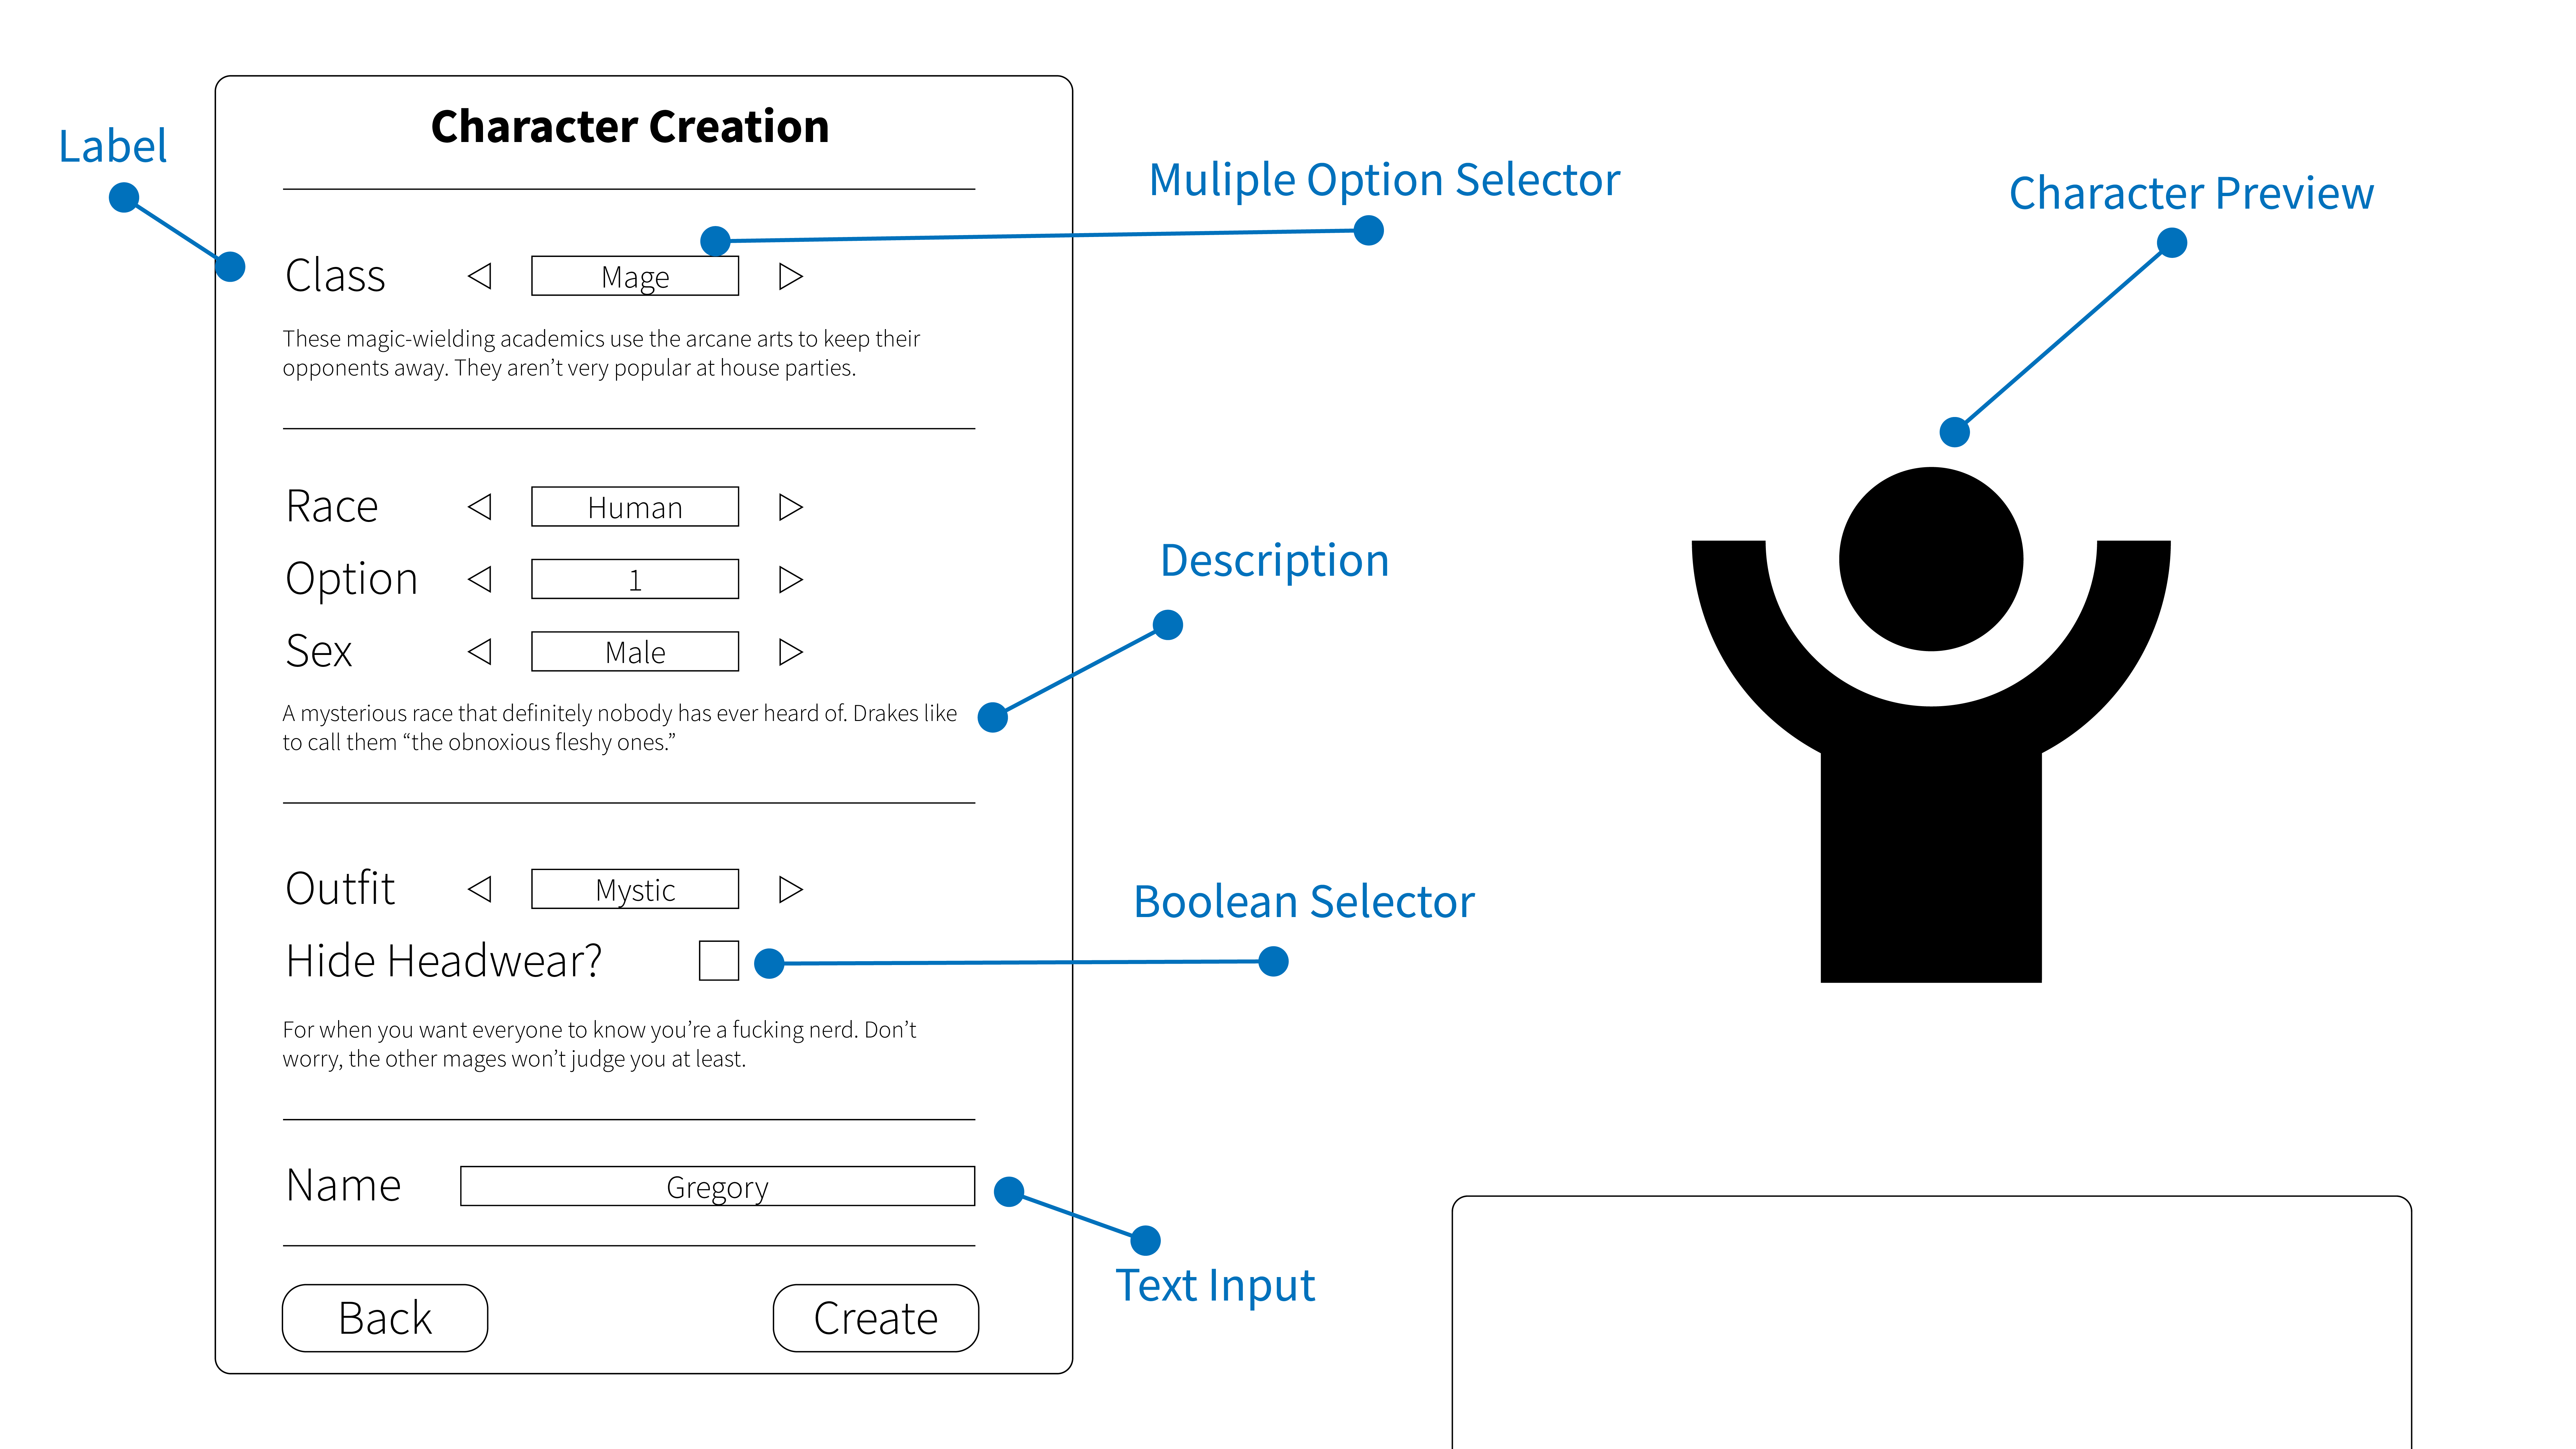
\includegraphics[width=1\linewidth]{images/character-creation.png}}
    \caption{The interface for creating or editing characters.}
\end{figure}

\subsection{Races and Body Sizes}

\begin{table}[h!]
    \centering
    \begin{tabular}{|c|c|c|}
    \hline
    \textbf{Small}  & \textbf{Medium} & \textbf{Large}   \\
    \hline
    Gnome  & Human  & Kong    \\
    \hline
    Dwarf  & Elf    & Troll   \\
    \hline
    Goblin & Orc    & Goliath \\
    \hline
    Corgo  & Purr   & Drake  \\
    \hline
    \end{tabular}
\end{table}

\pagebreak

\section{Flow}

\subsection{Match}

\paragraph{} Players who want to play a match start by choosing which rules they want to use. From there, they pick the stage first so another player cannot intentionally pick a stage their opponent's character is weaker on. Players will then select which character they want to use and start the match. Combat will largely consist of players blocking, dodging and attempting to find openings to exploit. If only one player remains with more than 0 HP or only one player did not get knocked out of the arena, they win the round. This will repeat until a player has won the majority of rounds. After that, players can change any of their previous selections, rematch or quit.


\subsection{State Machine}

\paragraph{} The game follows a simple state machine that is similar to other games. From the main menu, players can access the default play mode, the customization tools, the community organizing tool and basic settings. In the customization menu (referred to as the Locker Room), players can change their controls and customize their characters. In the community organizing tool, players can plan events, attend other peoples' events, manage their profiles and learn about news related to the game as well as the community. The settings menu allows players to adjust the basic aspects of the experience like audio levels, graphical quality and subtitles.

\begin{figure}[h!]
    \centering
    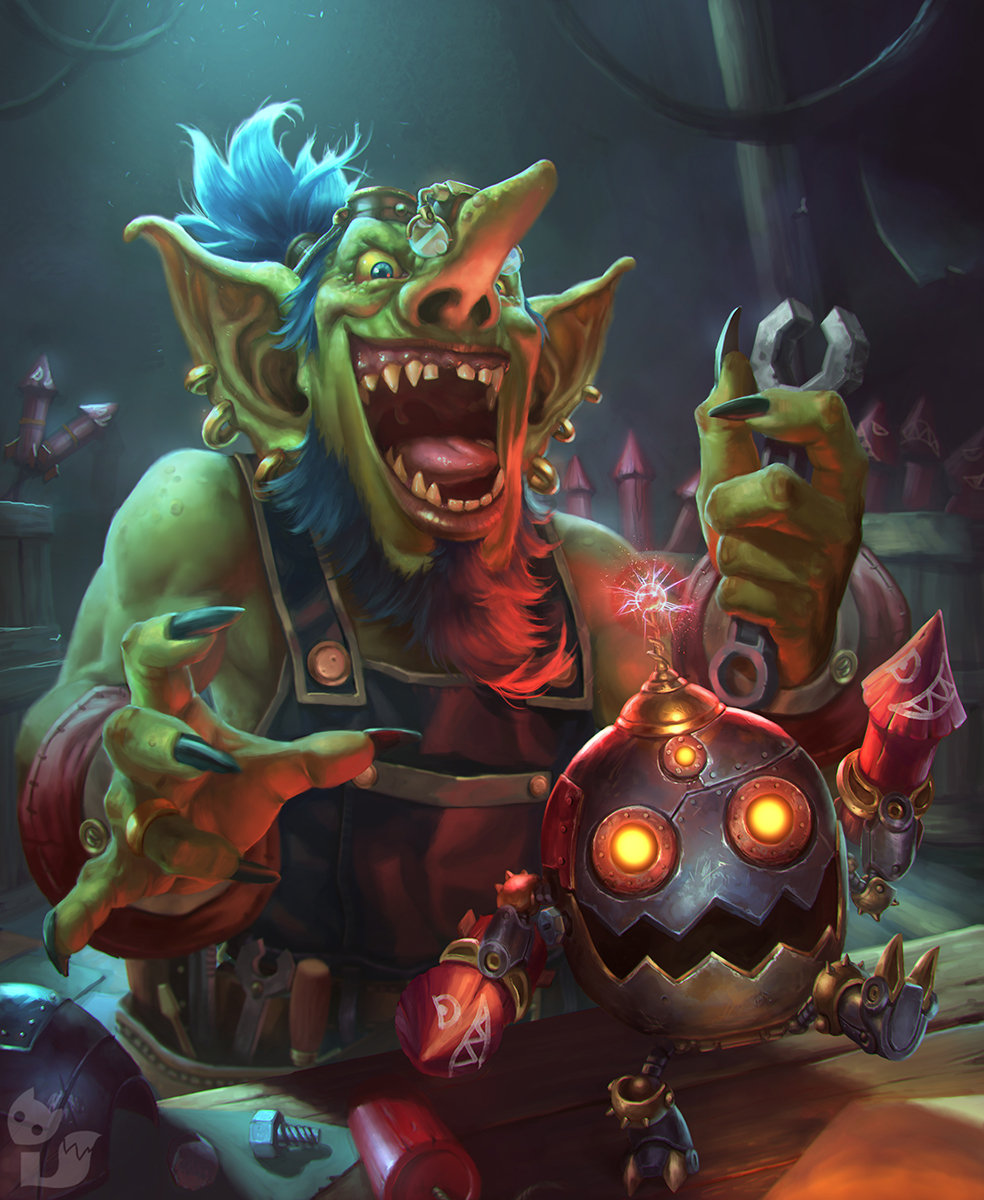
\includegraphics[width=0.5\linewidth]{images/characters-goblin.jpg}
    \caption{Mad Goblin Technician by Lie Setiawan.\nocite{setiawan_mad_2015}}
\end{figure}

\begin{figure}[h!]
    \centering
    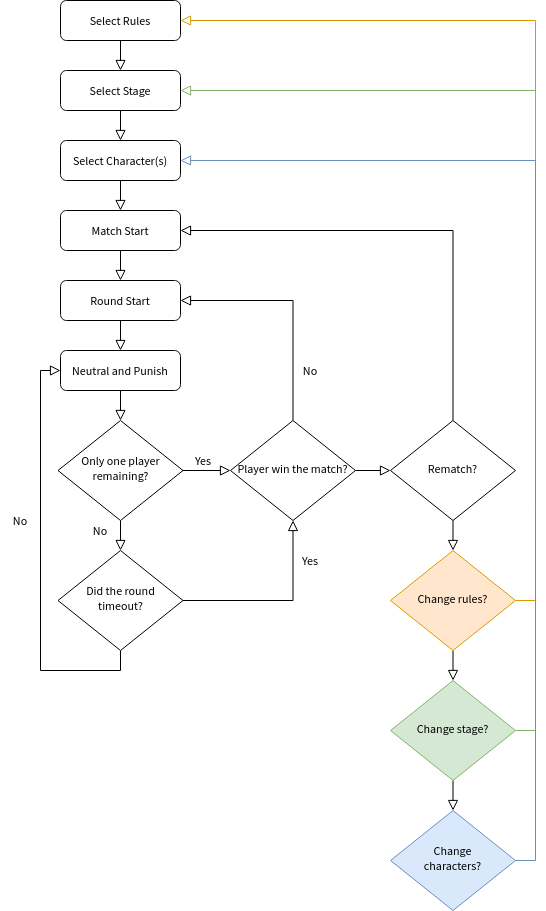
\includegraphics[width=.75\linewidth]{images/flow-match.png}
    \caption{The flow of the match from choosing the rules to choosing what happens when the set ends.}
\end{figure}

\pagebreak

\begin{figure}[h!]
    \centering
    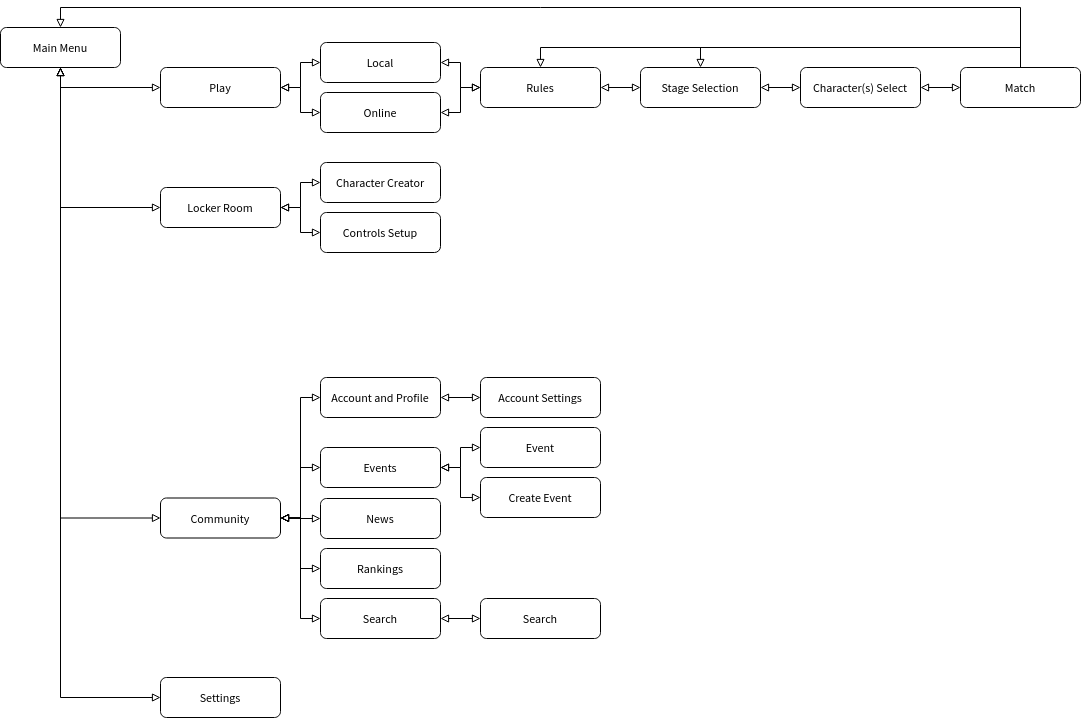
\includegraphics[width=1\linewidth]{images/flow-menu.png}
    \caption{The flow of the state machine and how players can navigate the menus.}
\end{figure}

\begin{figure}[h!]
    \centering
    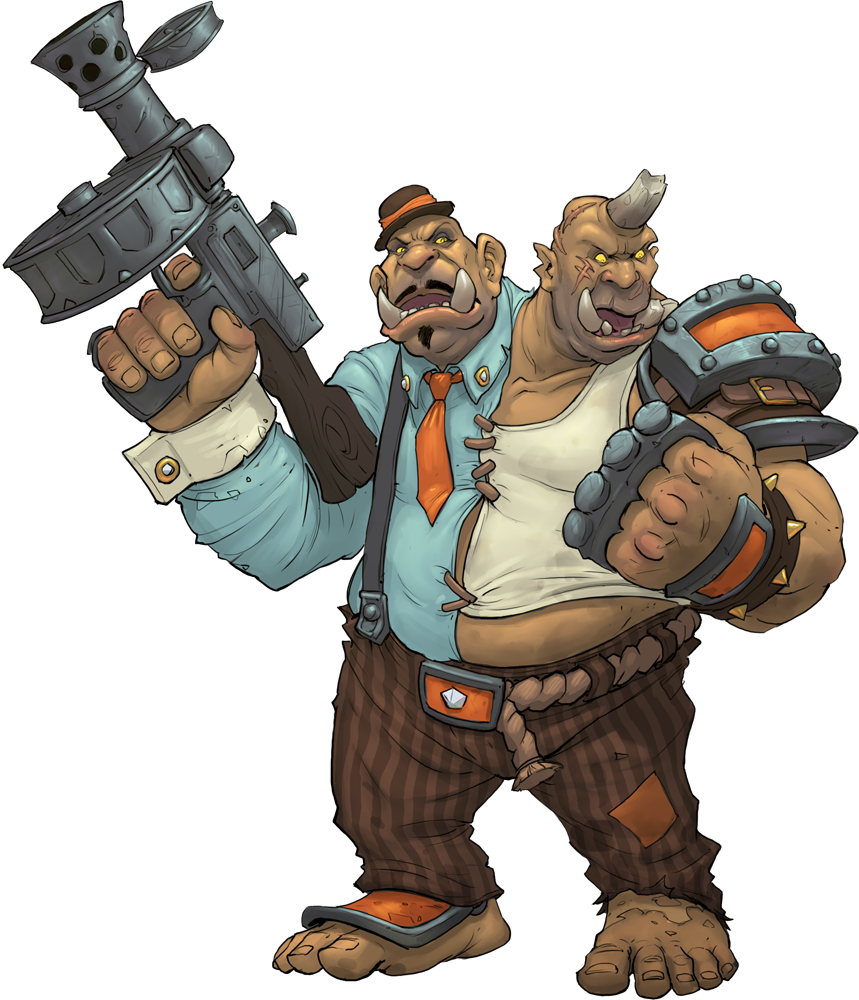
\includegraphics[width=0.3\linewidth]{images/characters-balance.png}
    \caption{Don Han-Cho by Blizzard Entertainment, Inc.\nocite{blizzard_entertainment_inc_don_2016}}
\end{figure}

\pagebreak

\section{Stages}

\paragraph{} OpenCombat has 5 stage layouts players can choose from. Each layout has advantages and disadvantages for certain classes but is selected before players pick their characters. All matches take place in the arena built by Mr. Peels but the aesthetic of the stage varies based on the time of day.

\subsection{No Platforms}

\paragraph{} This is the most basic stage with no platforms other than the stage itself. This layout has the most open space for combatants who want to move around freely or dominate a singular plane of combat. Combatants who can more effectively utilize platforms have difficulties on this layout but zoners and aerial combatants thrive here. Each player starts evenly spaced along the stage; if a player starts in the middle, it is advised that they find a way to not be trapped.

\begin{figure}[h!]
    \centering
    \fbox{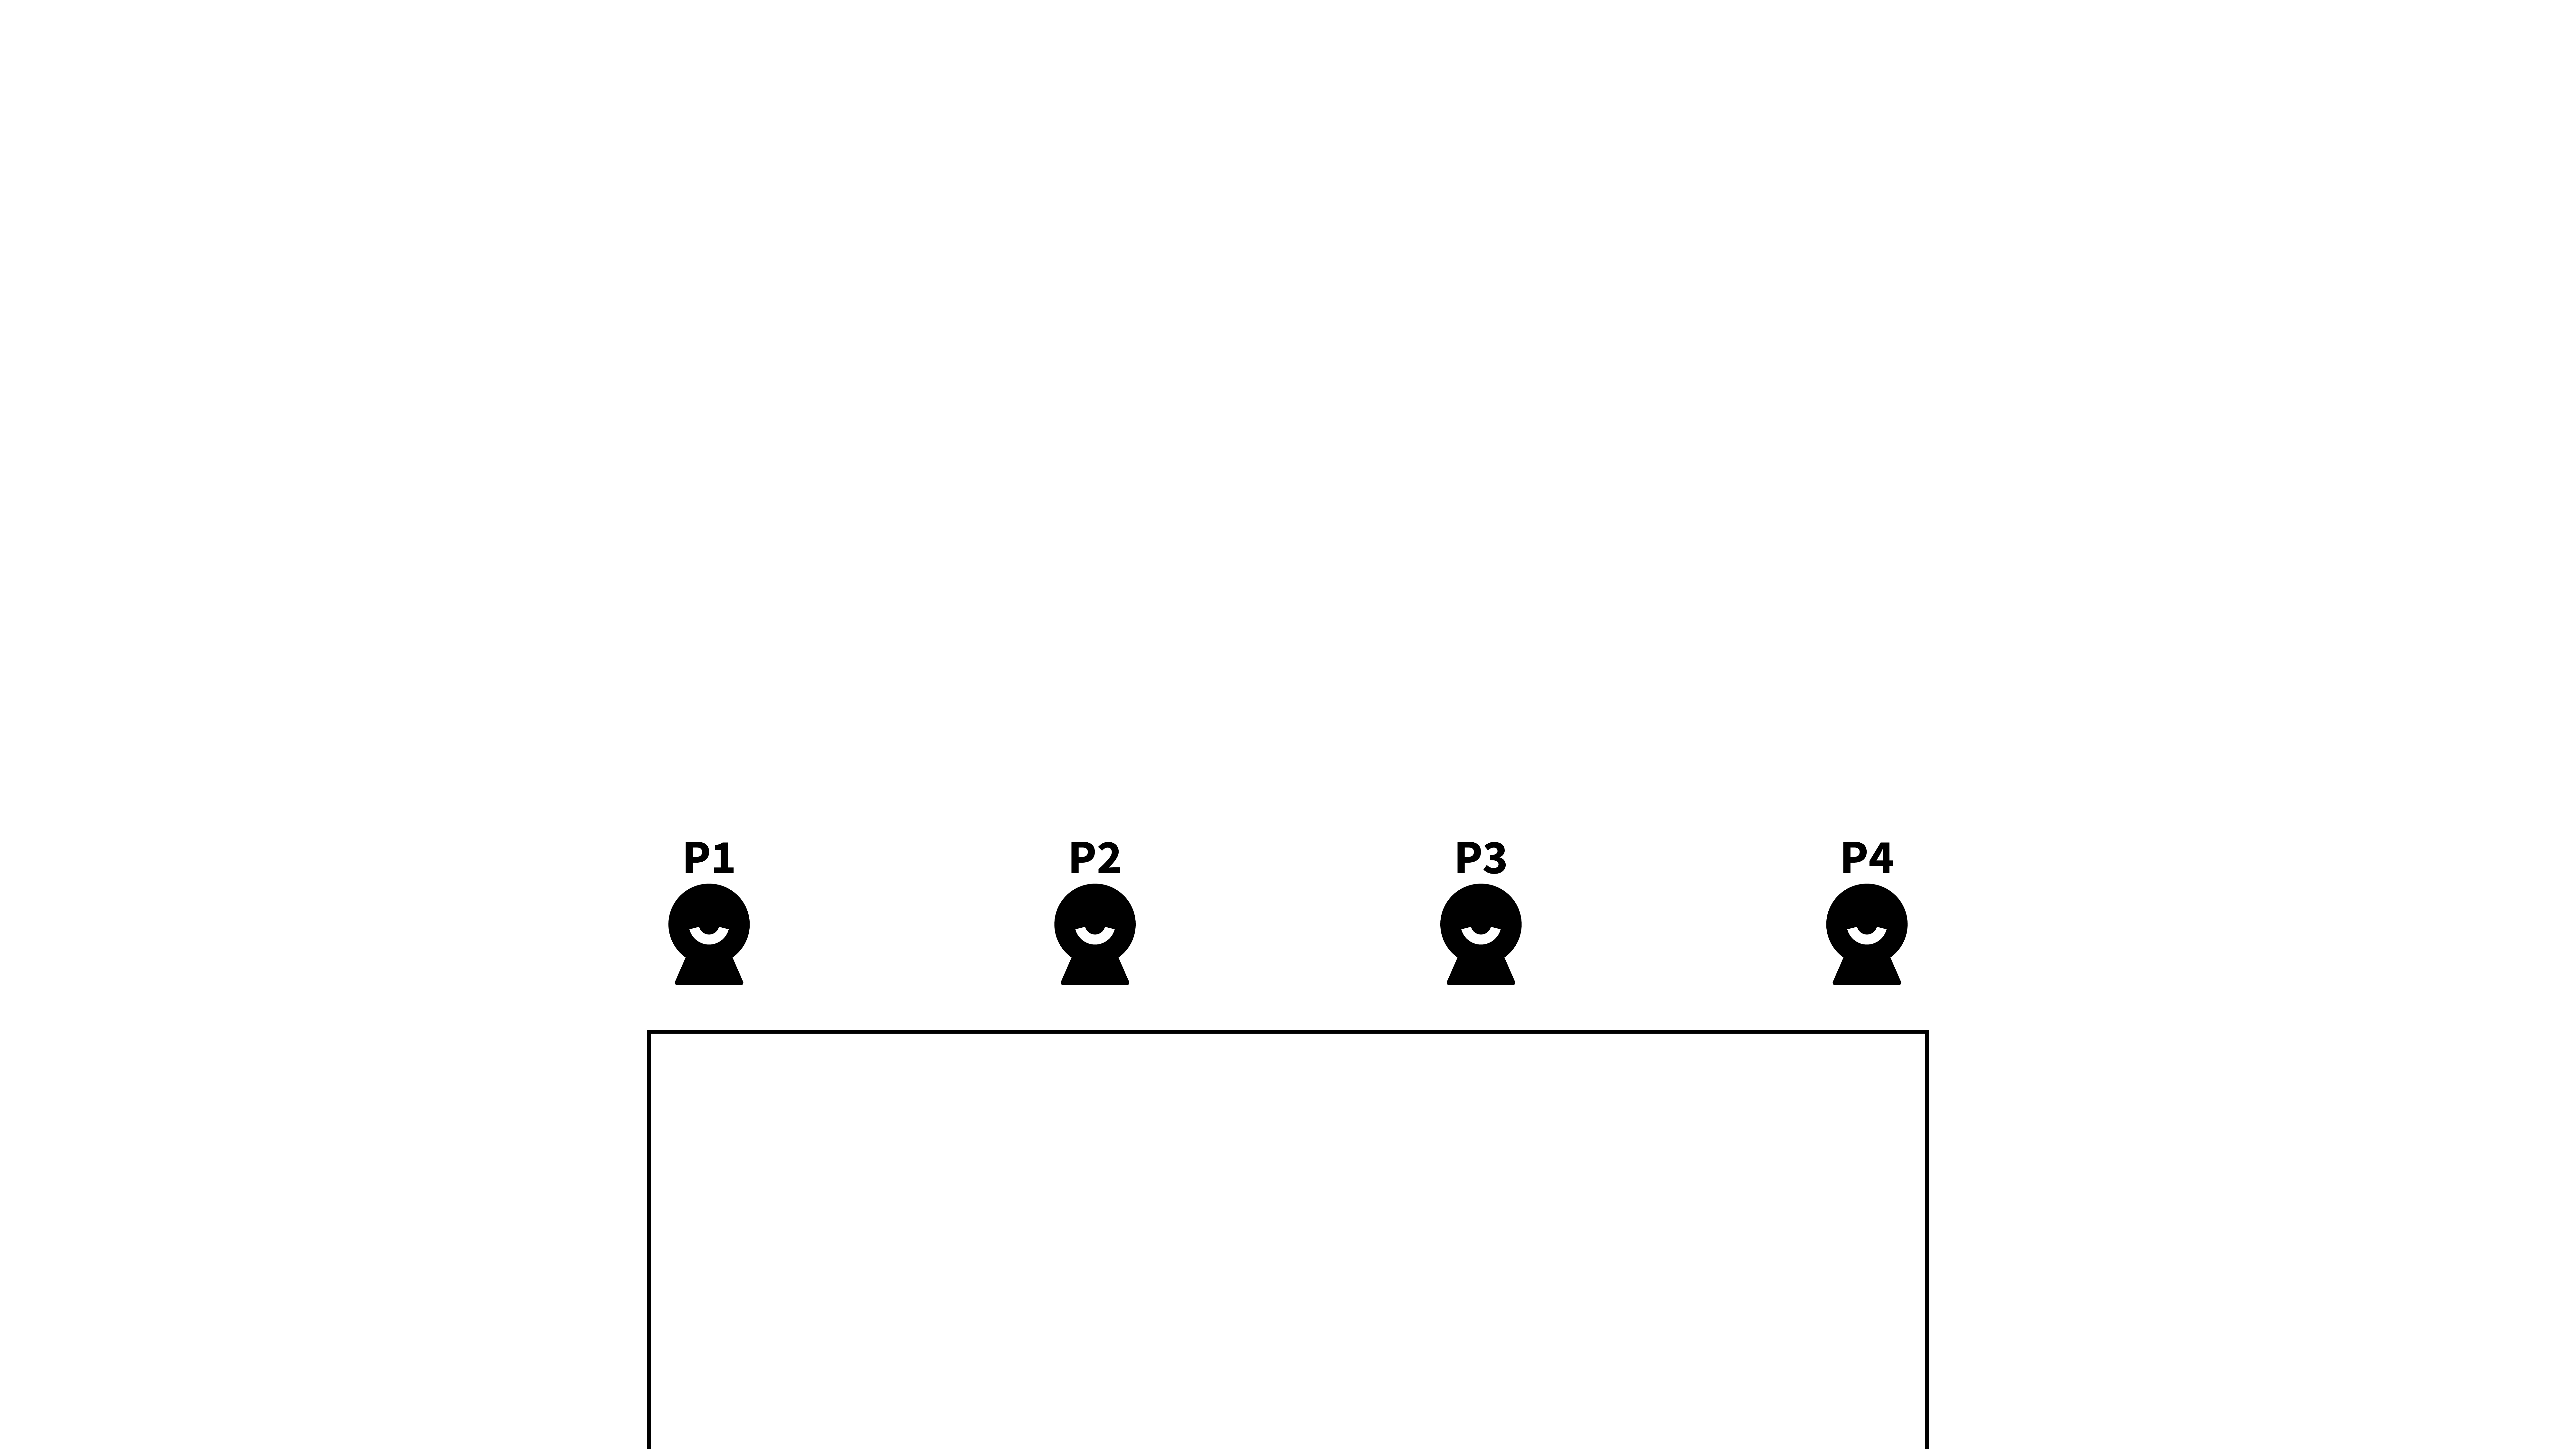
\includegraphics[width=1\linewidth]{images/levels-flat.png}}
    \caption{The most basic stage layout with no platforms and a lot of space to move around in.}
\end{figure}

\pagebreak

\subsection{Singular Platform}

\paragraph{} This layout features the basic flat stage plus one additional extended platform shortly above. Players can use the platform to chase their opponents in the air, continue a combo more easily or put themselves in a more advantageous position. Aerial characters excel at using this layout to juggle opponents around and slower characters with larger hitboxes on their attacks can trap their opponents on the platform easily. All players start on the stage itself, though, so it is advised to take control of the platform quickly if necessary.

\begin{figure}[h!]
    \centering
    \fbox{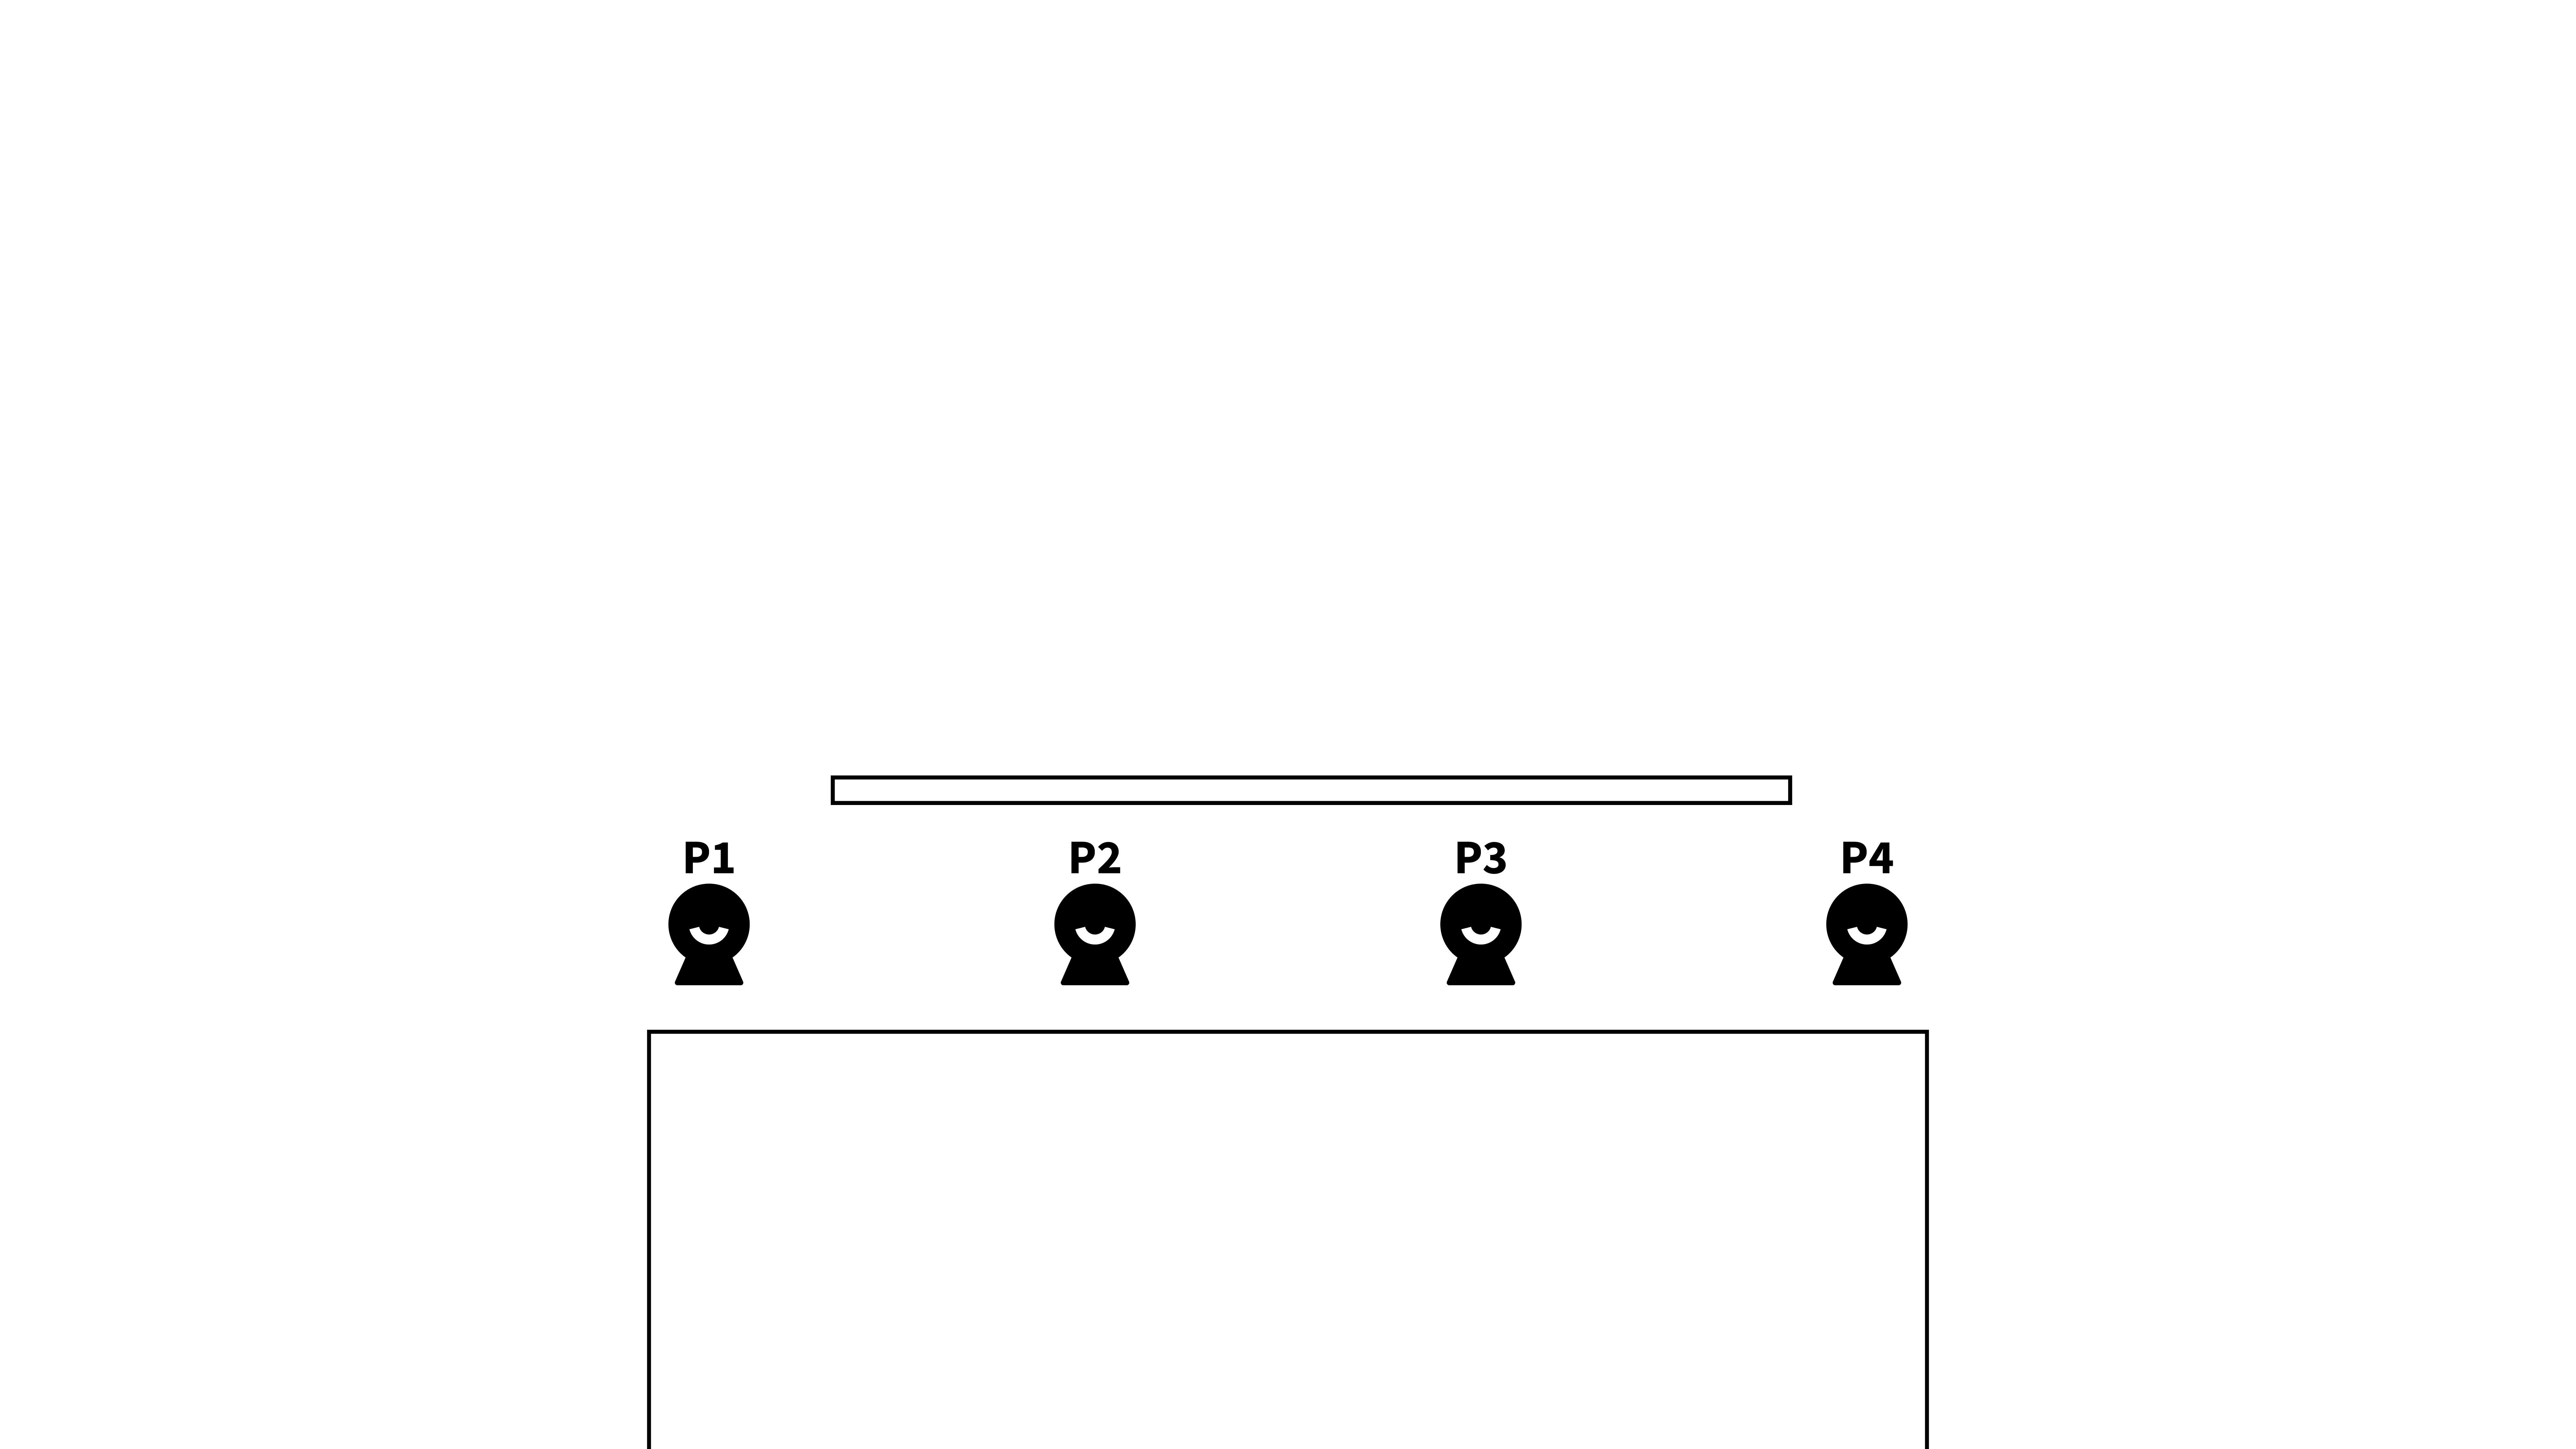
\includegraphics[width=1\linewidth]{images/levels-single.png}}
    \caption{The most notable component of this layout is the extended platform in the middle of the map that be used for positioning, juggling and set-ups.}
\end{figure}

\pagebreak

\subsection{Dual Platforms}

\paragraph{} Two platforms extend pass the edges of the stage on this layout with the middle being open. Fighters who want to knock their opponents out of the arena excel on this layout while slower characters struggle to navigate the openings the platforms create. The first two players start on the platforms, making 1v1 matches a scramble to control the center of the stage; matches with more than 2 players have the 3rd and 4th players starting on the stage itself.

\begin{figure}[h!]
    \centering
    \fbox{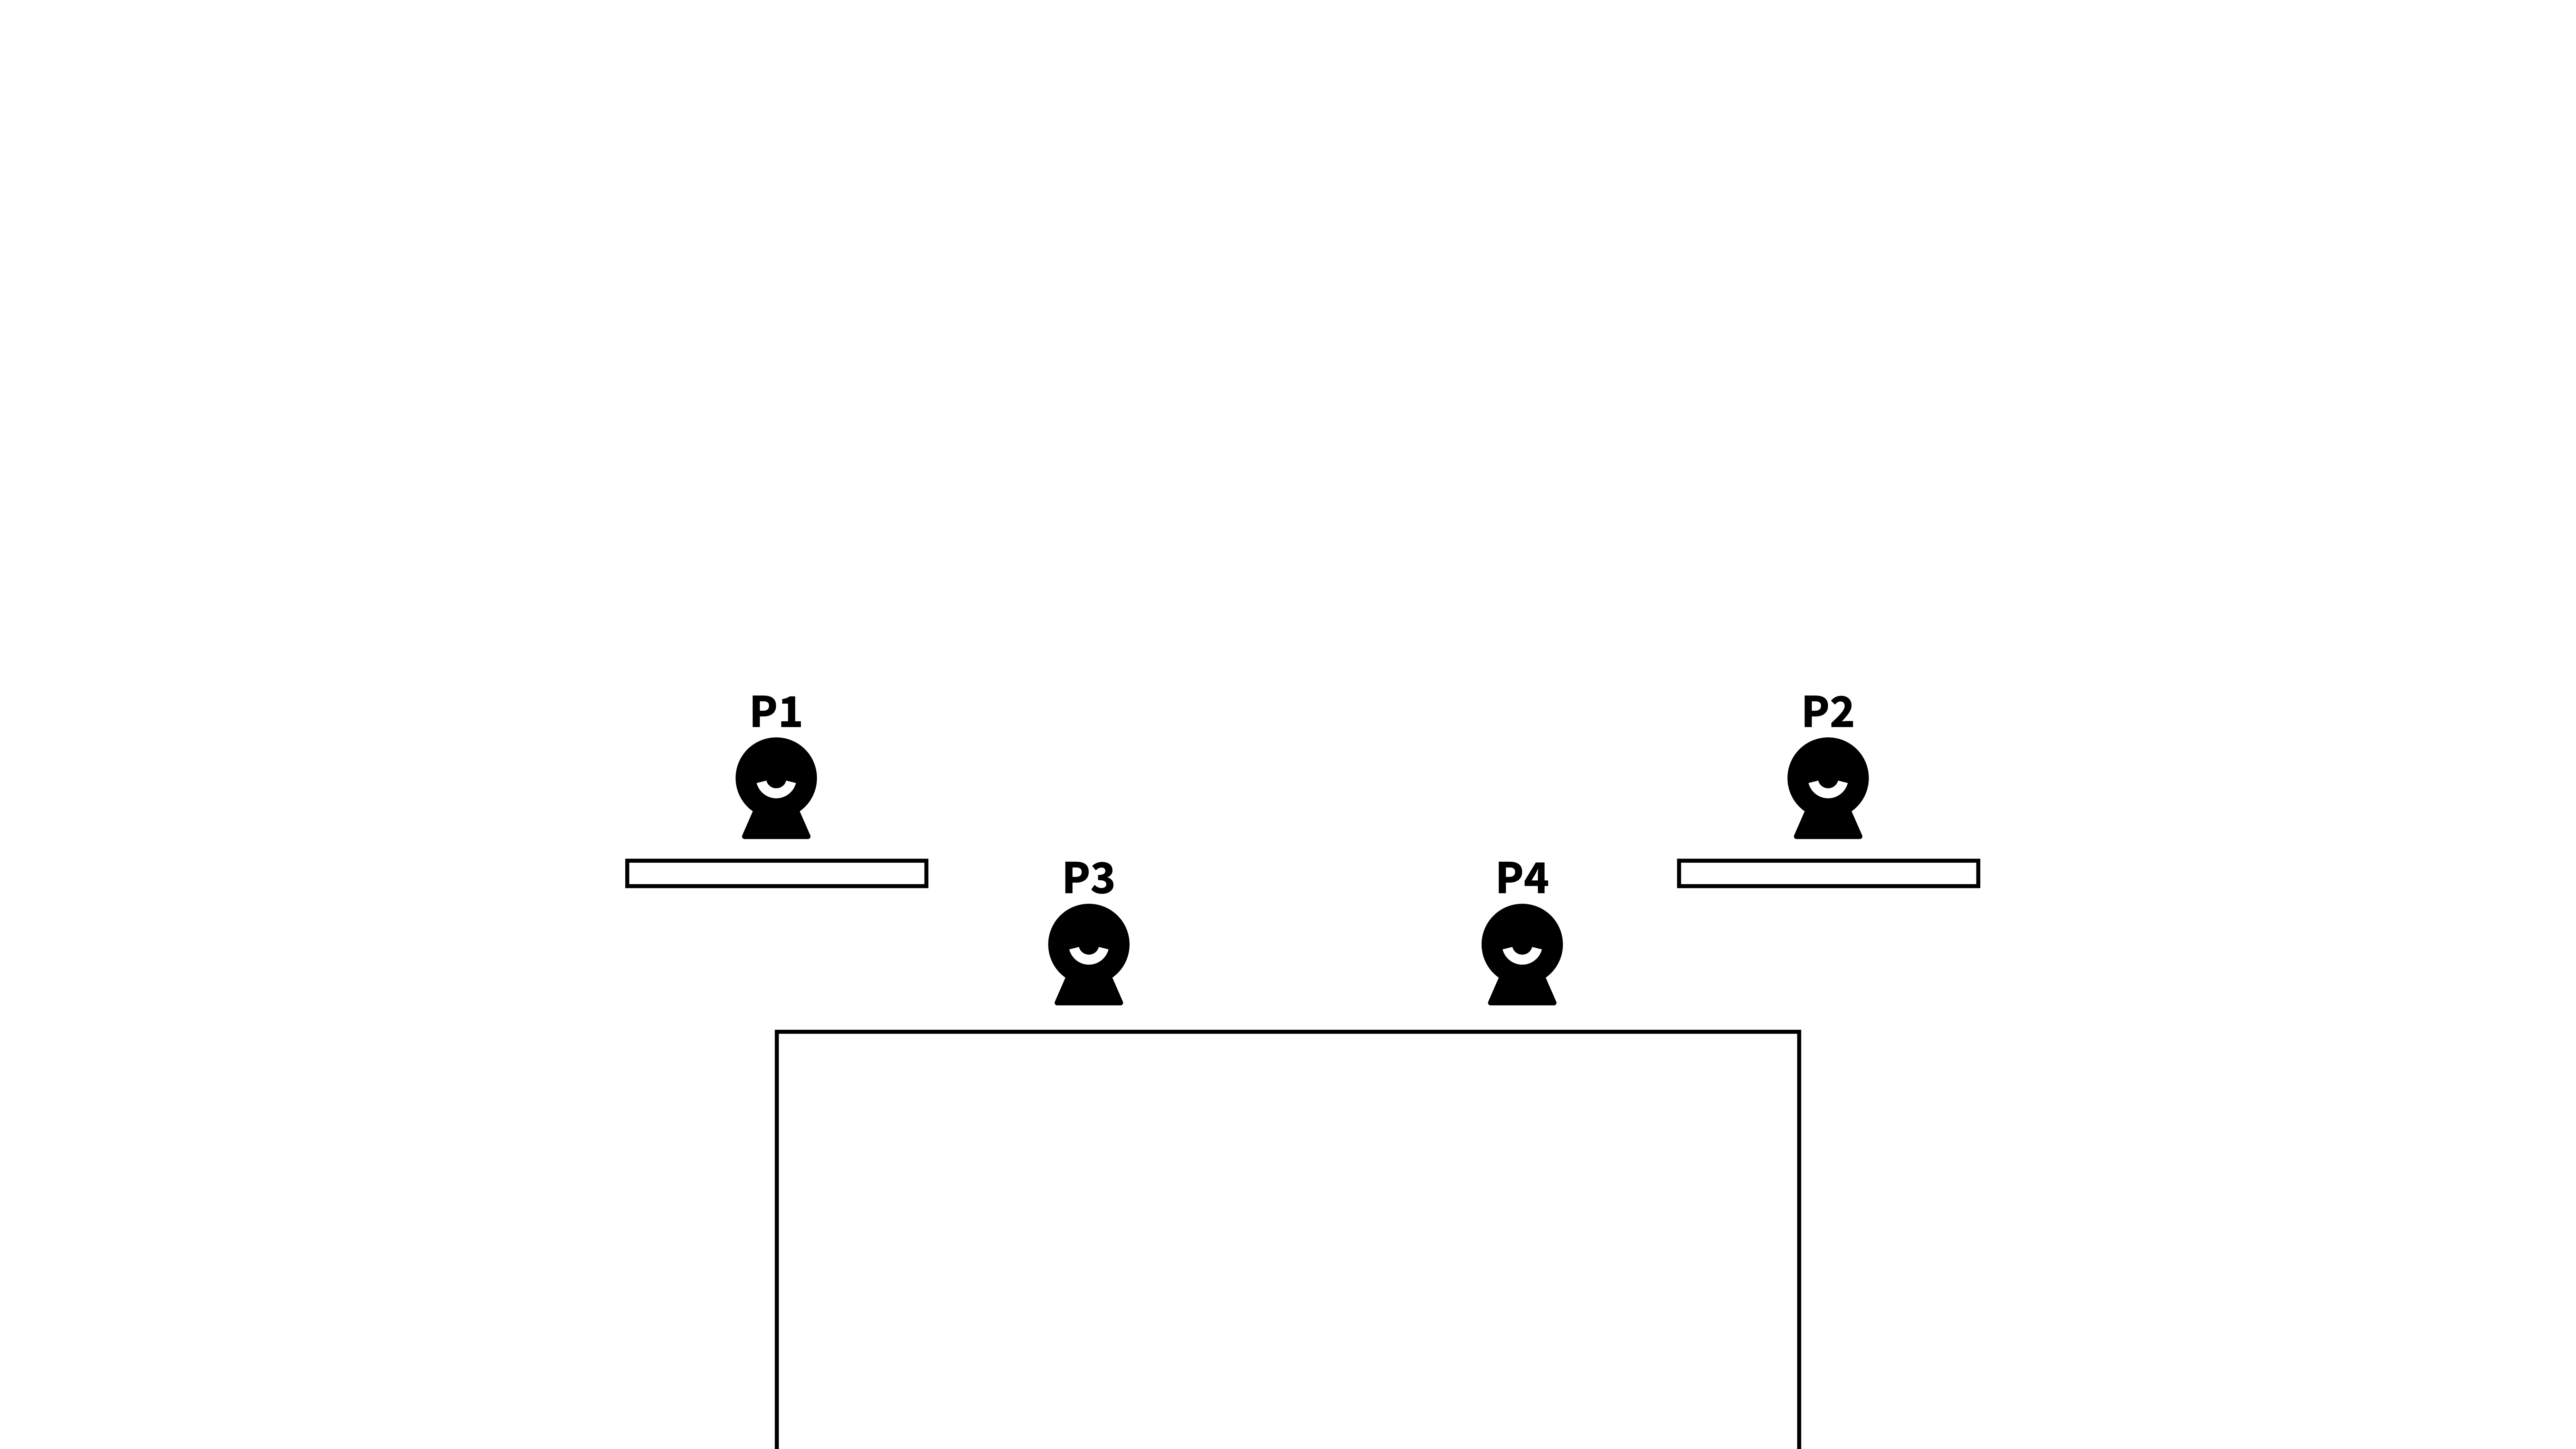
\includegraphics[width=1\linewidth]{images/levels-duo.png}}
    \caption{This layout has two platforms that extend off the edge of the stage. This is ideal for combatants who want to ring-out their opponents.}
\end{figure}

\pagebreak

\subsection{Triple Platforms}

\paragraph{} Players familiar with the Super Smash Bros. will be familiar with this layout which is inspired by the Battlefield stage featured in every game in the franchise since Melee. This stage traditional favors faster characters are the platforms allow them to close the distance between aerial and non-aerial opponents. Each player starts on either their own platform or the stage itself.

\begin{figure}[h!]
    \centering
    \fbox{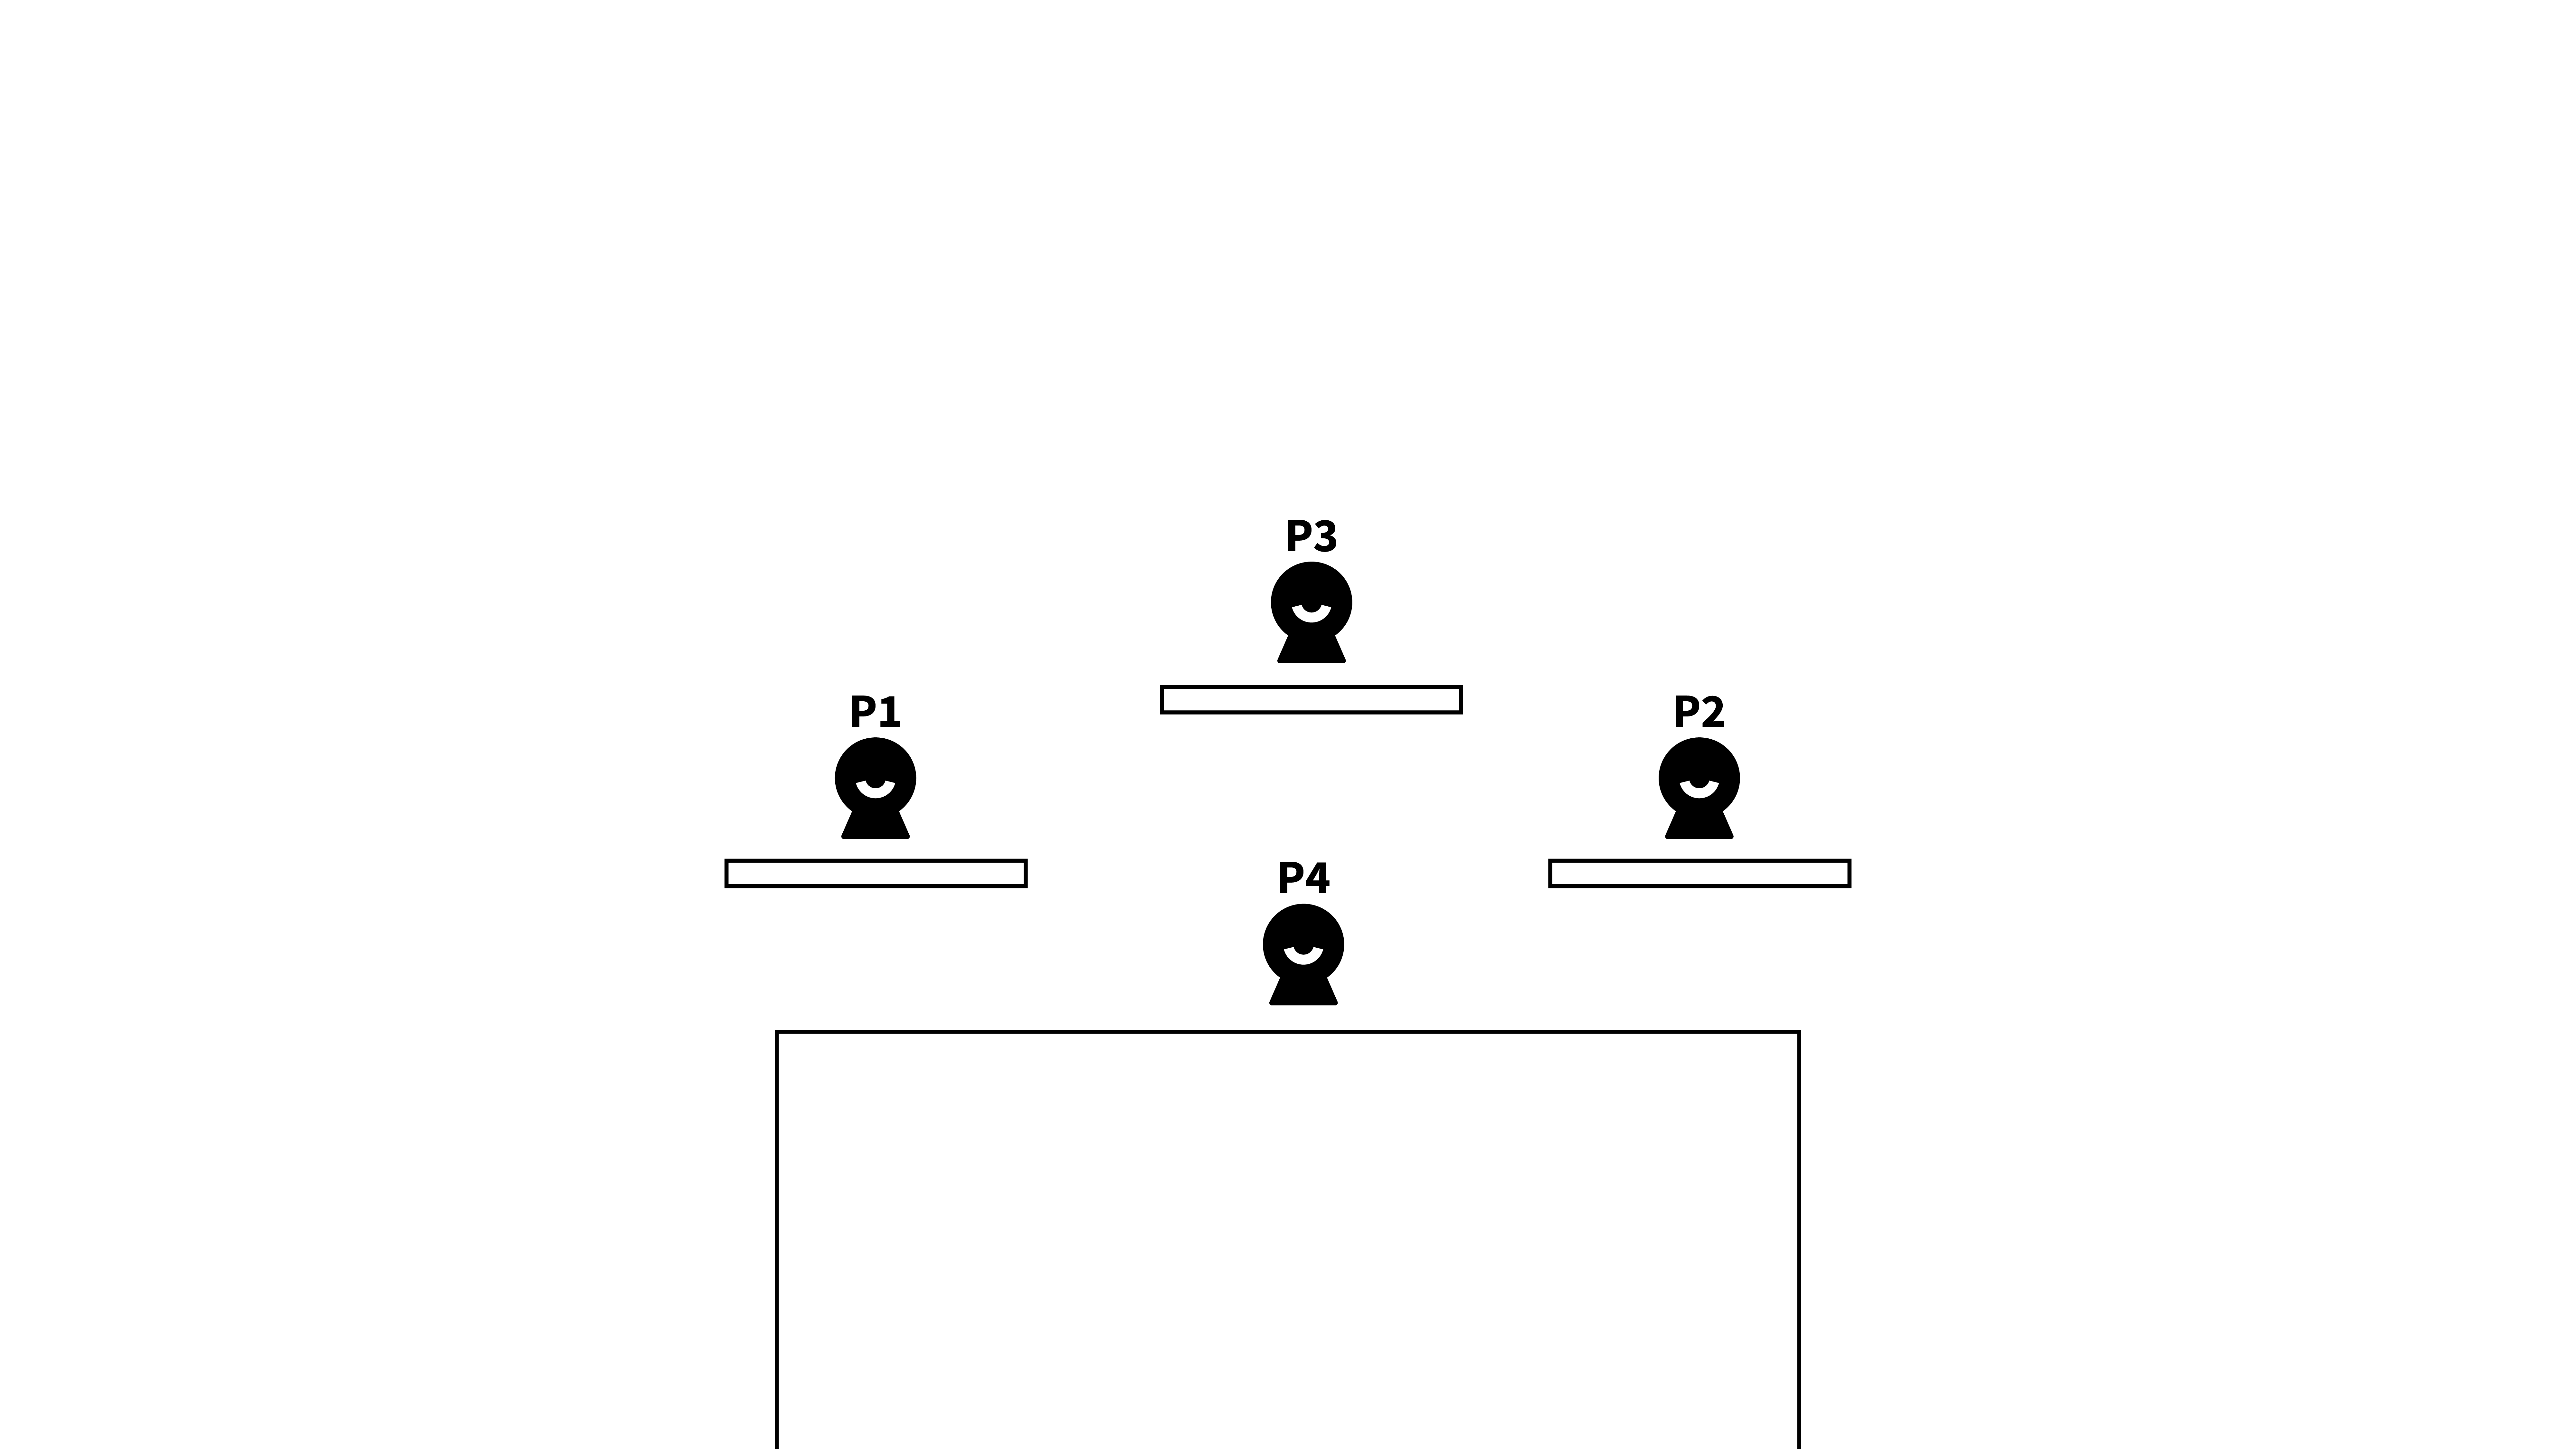
\includegraphics[width=1\linewidth]{images/levels-tri.png}}
    \caption{This layout features 3 small platforms in a triangular pattern above the stage.}
\end{figure}

\pagebreak

\subsection{Dual-Triple Combination}

\paragraph{} For some additional variety, players can also choose to fight on a stage that takes its layout from the singular and duo platform variants. Similar to the triple platform layout, this features three platforms in a triangular pattern but the middle platform is extended and the side platforms are on the edge of the stage. Combatants that can take advantage of mixed layouts like aerial or fast characters benefit the most from a layout like this. 

\begin{figure}[h!]
    \centering
    \fbox{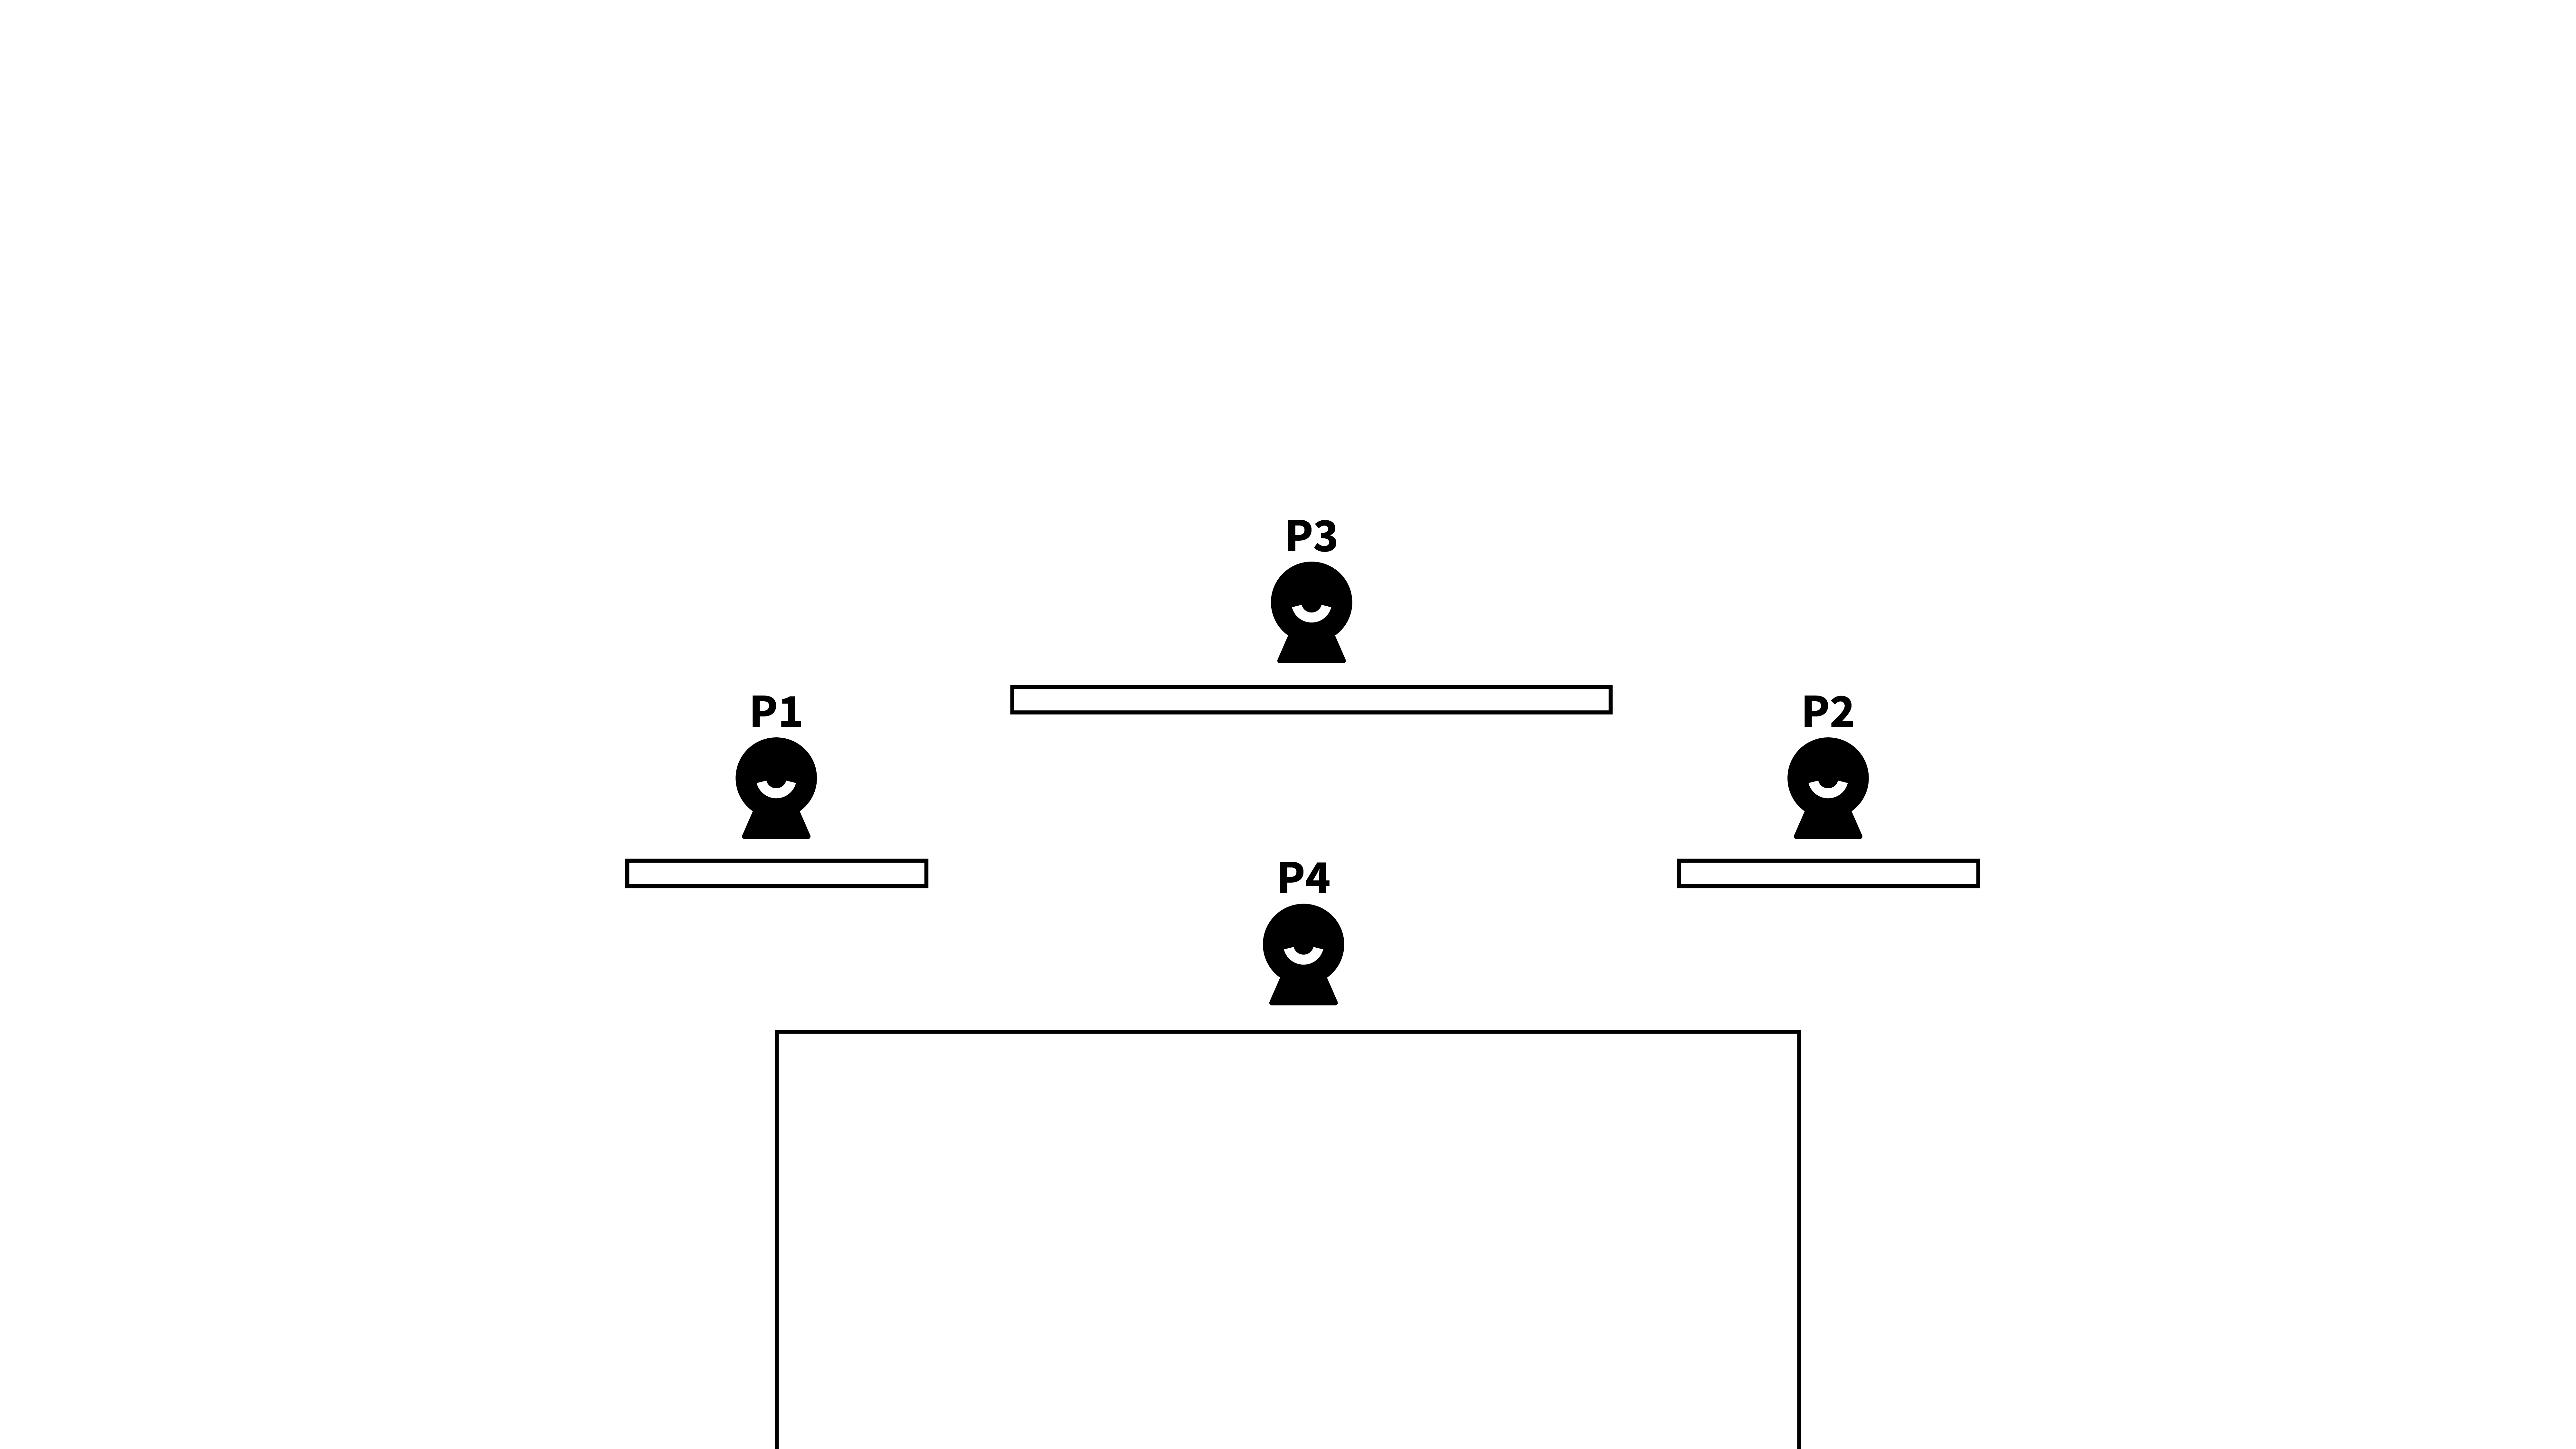
\includegraphics[width=1\linewidth]{images/levels-combo.png}}
    \caption{Both the extended platform from the singular variant and the edge platforms from the dual variant are included in this layout.}
\end{figure}